\documentclass[12pt,a4paper]{report}
\usepackage{cite}
\usepackage{amsmath,amssymb,amsfonts}
\usepackage{graphicx}
\graphicspath{{./}{figures/}{../../figures/}}
\usepackage{xcolor}
\usepackage{booktabs}
\usepackage{geometry}
\usepackage{tocloft}
\usepackage{setspace}
\usepackage{hyperref}

\geometry{top=2.5cm, bottom=2.5cm, left=3.0cm, right=2.5cm}
\onehalfspacing

\begin{document}

%----------------------------------------------------------------------------------------
% TITLE PAGE
%----------------------------------------------------------------------------------------
\begin{titlepage}
\thispagestyle{empty}
\begin{center}

{\Large\bfseries\color{blue} OUTREACH INTERNSHIP PROGRAM (2026)}\\[0.2cm]
{\large \textbf{PROJECT REPORT}}\\[0.4cm]

{\Huge\bfseries
An Adaptive Explainable Graph Digital Twin for Cyber-Resilient Smart Grids\\[0.2cm]
}

\rule{0.8\textwidth}{0.5pt}
\vspace{0.3cm}

{\large\textbf{Submitted by}}\\[0.2cm]
{\Large\bfseries
Anshika Keshari
}\\[0.1cm]
OIP ID: 20260084\\
Department of Computer Science and Engineering\\
Kalinga Institute of Industrial Technology, Bhubaneswar

\vspace{0.4cm}

{\large\textbf{Under the Guidance of}}\\[0.2cm]
{\large
Mr. Mallikharjuna Rao K\\
Assistant Professor\\
International Institute of Information Technology, Naya Raipur
}

\vspace{1.1cm}

% Logos
\begin{minipage}{0.45\textwidth}
\centering
% \includegraphics[width=4.0cm]{iiitnr_logo.png} % TODO: Replace with real logo image
\vspace{1.5cm}
\textbf{IIIT Naya Raipur}
\end{minipage}
\hfill
\begin{minipage}{0.45\textwidth}
\centering
% \includegraphics[width=4.0cm]{kiit_logo.png} % TODO: Replace with real logo image
\vspace{1.5cm}
\textbf{KIIT Bhubaneswar}
\end{minipage}

\vspace{0.8cm}
\textbf{Department of Computer Science and Engineering}\\
{\small Kalinga Institute of Industrial Technology, Bhubaneswar, Odisha, India}

\vspace{0.4cm}
{\large\bfseries May - July 2026}

\end{center}
\end{titlepage}

%----------------------------------------------------------------------------------------
% ACKNOWLEDGEMENT
%----------------------------------------------------------------------------------------
\thispagestyle{empty}
\vspace*{1.5cm}
\begin{center}
    {\Huge \textbf{ACKNOWLEDGEMENT}}
\end{center}
\vspace{1cm}

I wish to convey my sincere appreciation and gratitude to my research supervisor, \textbf{Mr. Mallikharjuna Rao K}, Department of Computer Science and Engineering, International Institute of Information Technology, Naya Raipur, for his constant mentorship, technical insights, and encouragement throughout the course of this internship. His guidance was crucial in helping me understand the physical and cyber-physical intricacies of smart grid systems.

\vspace{0.6cm}
I am also highly grateful to the academic administration of the \textbf{International Institute of Information Technology, Naya Raipur} for providing the research facilities, computational resources, and a stimulating academic environment that made the completion of this project possible.

\vspace{0.6cm}
I must also extend my heartfelt thanks to my parents and friends for their continuous support, patience, and encouragement during this research work.

\vspace{1.5cm}
\noindent
\begin{minipage}[t]{0.45\textwidth}
\raggedright
Date: \\[0.4cm]
Place: Bhubaneswar
\end{minipage}
\hfill
\begin{minipage}[t]{0.5\textwidth}
\centering
\rule{6cm}{0.4pt} \\[0.2cm]
\textbf{Anshika Keshari}
\end{minipage}

%----------------------------------------------------------------------------------------
% DECLARATION
%----------------------------------------------------------------------------------------
\newpage
\thispagestyle{empty}
\vspace*{1.5cm}
\begin{center}
    {\Huge\bfseries DECLARATION}
\end{center}
\vspace{1.5cm}

I hereby declare that the project report entitled \textbf{``AN ADAPTIVE EXPLAINABLE GRAPH DIGITAL TWIN FOR CYBER-RESILIENT SMART GRIDS''} is an original research work carried out by me during the Outreach Internship Program (OIP) 2026 under the joint guidance of \textbf{Mr. Mallikharjuna Rao K}, Department of Computer Science and Engineering, International Institute of Information Technology, Naya Raipur.

This report is submitted in partial fulfillment of the internship requirements and has not been submitted, in part or in full, to any other institution or university for the award of any other degree or diploma. All the literature and data sources utilized in this work have been duly cited and acknowledged.

\vspace{3cm}
\noindent
\begin{minipage}[t]{0.45\textwidth}
\raggedright
Date: \\[0.4cm]
Place: Bhubaneswar
\end{minipage}
\hfill
\begin{minipage}[t]{0.5\textwidth}
\centering
\rule{6cm}{0.4pt} \\[0.2cm]
\textbf{Anshika Keshari} \\
OIP ID: 20260084 \\
Department of Computer Science and Engineering \\
Kalinga Institute of Industrial Technology, Bhubaneswar
\end{minipage}

%----------------------------------------------------------------------------------------
% CERTIFICATE
%----------------------------------------------------------------------------------------
\newpage
\thispagestyle{empty}
\vspace*{2cm}
\begin{center}
    {\Huge \textbf{CERTIFICATE}}
\end{center}
\vspace{1.5cm}

This is to certify that the comprehensive report titled ``\textbf{AN ADAPTIVE EXPLAINABLE GRAPH DIGITAL TWIN FOR CYBER-RESILIENT SMART GRIDS}'' submitted by \textbf{Anshika Keshari} from \textbf{Kalinga Institute of Industrial Technology, Bhubaneswar} at \textbf{IIIT-NR OIP 2026} is a record of original research work carried out by her under my direct supervision and guidance.

\vspace{4cm}
\hfill
\begin{minipage}{0.45\textwidth}
    \centering
    \rule{7cm}{0.4pt} \\
    \vspace{0.3cm}
    \textbf{Submitted to:} \\
    \vspace{0.2cm}
    Mr. Mallikharjuna Rao K \\
    Assistant Professor \\
    IIIT-NR
\end{minipage}

%----------------------------------------------------------------------------------------
% TABLE OF CONTENTS
%----------------------------------------------------------------------------------------
\newpage
\pagenumbering{roman}
\tableofcontents
\newpage
\pagenumbering{arabic}

%----------------------------------------------------------------------------------------
% CHAPTER 1: INTRODUCTION
%----------------------------------------------------------------------------------------
\chapter{Introduction}
Modern electrical grids have transitioned from isolated analog systems into highly interconnected cyber-physical networks. By integrating Supervisory Control and Data Acquisition (SCADA) systems, phasor measurement units (PMUs), and automated smart sensors, utilities can monitor wide-area transmission lines in real time. However, this tight integration between physical power lines and digital communications opens up new vectors for malicious cyber-attacks.

Among these threats, False Data Injection Attacks (FDIAs) are particularly dangerous. Unlike raw denial-of-service attacks that disrupt communications, a stealthy FDIA alters sensor readings in a coordinated manner. The attacker exploits knowledge of the physical system's topology and admittance parameters to modify telemetry values (voltage magnitudes, active power flows) while satisfying Kirchhoff's circuit laws. As a result, the corrupted telemetry successfully passes through classical state estimation Bad Data Detection (BDD) filters, which rely on static measurement residuals. The control center then receives manipulated states, leading to incorrect generation dispatch commands, economic losses, or physical line trips.

To resolve these challenges, this project introduces a Graph Digital Twin (GDT) framework that couples a dynamic virtual model of the electrical network with a multi-task GraphSAGE neural network. GNNs are ideal for smart grids because the physical layout of buses and transmission lines directly maps to a graph structure. Unlike traditional machine learning models (like MLPs) that require a fixed input dimension, a GNN operates on variable graph topologies. When a line outage occurs and the network reconfigures, the GNN adapts dynamically. 

\section{Research Gap}
Conventional cyber-security schemes suffer from several critical gaps:
\begin{itemize}
    \item \textbf{Fixed Topology Limitations}: Traditional classifiers like Multi-Layer Perceptrons (MLPs) assume static network inputs. A scheduled line outage or transformer trip alters the spatial layout of measurements, forcing the MLP to experience dimension errors unless the entire model is retrained.
    \item \textbf{Over-smoothing in Isotropic GNNs}: Early GNN architectures (such as Graph Convolutional Networks) aggregate neighborhood states using uniform spatial averaging. Over multiple message-passing layers, this averages out node-level feature details, leading to over-smoothing and severely degrading the model's ability to localize which specific bus is under attack.
    \item \textbf{Open-loop Alarms}: Most existing ML methods act as open-loop detectors. They raise an alarm when an attack occurs, but offer no explanation of the attack vector or any self-healing control actions to restore the true state estimation.
\end{itemize}

\section{Main Contributions}
The main contributions of this project report are summarized as follows:
\begin{itemize}
    \item We propose a physics-conforming Graph Digital Twin (GDT) framework that integrates AC power flow physics with a joint multi-task GraphSAGE neural network to concurrently detect grid-level FDIAs and localize compromised buses.
    \item We leverage GraphSAGE's concatenation-based convolution to preserve node-level feature signatures, preventing over-smoothing and enabling high-precision target localization.
    \item We integrate the Integrated Gradients (IG) explainability method, providing mathematically rigorous, sensor-level feature attributions to trace the attack vectors.
    \item We implement a closed-loop grid healing module that isolates compromised telemetry channels and substitutes forecasted baseline nominal estimates to restore tracking accuracy.
    \item We benchmark the framework against classical Weighted Least Squares (WLS) state estimators and validate its cross-grid inductive transfer learning on the IEEE 30-bus system.
\end{itemize}

%----------------------------------------------------------------------------------------
% CHAPTER 2: LITERATURE REVIEW
%----------------------------------------------------------------------------------------
\chapter{Literature Review}
Cyber-physical security in smart grids has been a major research focus since the pioneering work of Liu et al. \cite{b3}, who proved that an attacker with knowledge of the network Jacobian matrix could construct stealthy FDIAs that bypass state estimation BDD filters. 

To combat this, researchers initially proposed mathematical state estimation defenses. Zhao and Mili \cite{b5} proposed robust estimators to mitigate malicious telemetry corruption. However, these methods require significant computational overhead and struggle when multiple sensors are compromised.

In recent years, machine learning models have been extensively studied. Early attempts focused on flat classifiers such as Support Vector Machines (SVMs) and MLPs. However, these models cannot handle topological changes. If a line is tripped, the input vector size changes, causing the model to crash. 

To overcome this, Graph Neural Networks (GNNs) were introduced. Boyaci et al. \cite{b10} developed a joint detection and localization scheme using ARMA GNNs. While ARMA filters capture localized structural information, they are computationally heavy during training. Yue and Qu \cite{b14} proposed a Graph Convolutional Network (GCN) approach for attack detection, but their model was evaluated on a static grid and did not address localized node anomalies or over-smoothing.

Explainable AI (XAI) is critical for operator trust in smart grids. Most GNN explainers (such as GNNExplainer \cite{b15} or perturbation-based LIME/SHAP) are heuristic. They perturb the input features randomly to observe output changes. However, this process is computationally expensive and does not satisfy the completeness axiom, meaning the attributions do not sum to the model's output prediction difference. This project bridges these gaps by deploying a dynamic Graph Digital Twin coupled with Integrated Gradients explainability and closed-loop mitigation.

%----------------------------------------------------------------------------------------
% CHAPTER 3: MATHEMATICAL MODELING
%----------------------------------------------------------------------------------------
\chapter{Mathematical Modeling}
We represent the electrical power grid as a spatial graph $G = (V, E)$, where $V$ represents the set of buses (substations) and $E$ represents the set of transmission lines and transformers.

\section{Node and Edge Mapping under AC Power Flow}
For each bus $i \in V$, the state vector $X_i \in \mathbb{R}^4$ is constructed from physical SCADA telemetry measurements:
\begin{equation}
X_i = [V_i, \theta_i, P_i, Q_i]^T
\end{equation}
where $V_i$ is the voltage magnitude in per-unit (p.u.), $\theta_i$ is the voltage angle in degrees, $P_i$ is the net active power injection (MW), and $Q_i$ is the net reactive power injection (MVAR). 

The transmission branch connections are represented by edge indices $E$. Each edge is mapped to a physical attribute vector $E_{attr} \in \mathbb{R}^2$ containing the branch resistance and reactance:
\begin{equation}
E_{attr, ij} = [R_{ij}, X_{ij}]^T
\end{equation}

Under non-linear AC power flow conditions, the power injections at each bus $i$ must satisfy Kirchhoff's current laws:
\begin{equation}
P_i = V_i \sum_{j \in \mathcal{N}(i)} V_j \left( G_{ij} \cos(\theta_i - \theta_j) + B_{ij} \sin(\theta_i - \theta_j) \right)
\end{equation}
\begin{equation}
Q_i = V_i \sum_{j \in \mathcal{N}(i)} V_j \left( G_{ij} \sin(\theta_i - \theta_j) - B_{ij} \cos(\theta_i - \theta_j) \right)
\end{equation}
where $G_{ij}$ and $B_{ij}$ are the conductance and susceptance parameters of the transmission line between bus $i$ and $j$.

\section{Stealthy False Data Injection Attacks (FDIAs)}
An attacker aims to inject a false vector $a$ into the sensor telemetry $z$ such that:
\begin{equation}
z' = z + a
\end{equation}
where $z'$ is the corrupted measurement vector. In a classical Weighted Least Squares (WLS) state estimator, the state tracking vector is computed by solving the non-linear optimization:
\begin{equation}
\min_x J(x) = [z - h(x)]^T R^{-1} [z - h(x)]
\end{equation}
where $h(x)$ is the non-linear measurement function and $R$ is the sensor noise covariance. The standard bad data detection (BDD) checks the measurement residual:
\begin{equation}
r = z - h(\hat{x})
\end{equation}
If the attacker constructs the attack vector $a$ to satisfy the physical grid equations ($a = h(x+c) - h(x)$), the estimated state shifts by $c$, but the residual remains unchanged:
\begin{equation}
r' = z' - h(\hat{x} + c) = z + h(x+c) - h(x) - h(\hat{x} + c) \approx z - h(\hat{x}) = r
\end{equation}
Thus, the residual does not exceed the Chi-square ($\chi^2$) threshold, and the attack completely bypasses the classical SCADA BDD filter.

%----------------------------------------------------------------------------------------
% CHAPTER 4: PROPOSED GRAPH DIGITAL TWIN ARCHITECTURE
%----------------------------------------------------------------------------------------
\chapter{Proposed Graph Digital Twin Architecture}
The proposed Graph Digital Twin (GDT) framework establishes a synchronized digital replica of the physical grid. The architecture consists of three main modules: the virtual replica data pipeline, the multi-task GraphSAGE neural network, and the explainable self-healing control system. The detailed interaction is mapped in Figure \ref{fig:architecture}.

\begin{figure}[htbp]
\centering
% Note: In LaTeX compile, this references the gdt_architecture.png generated by python
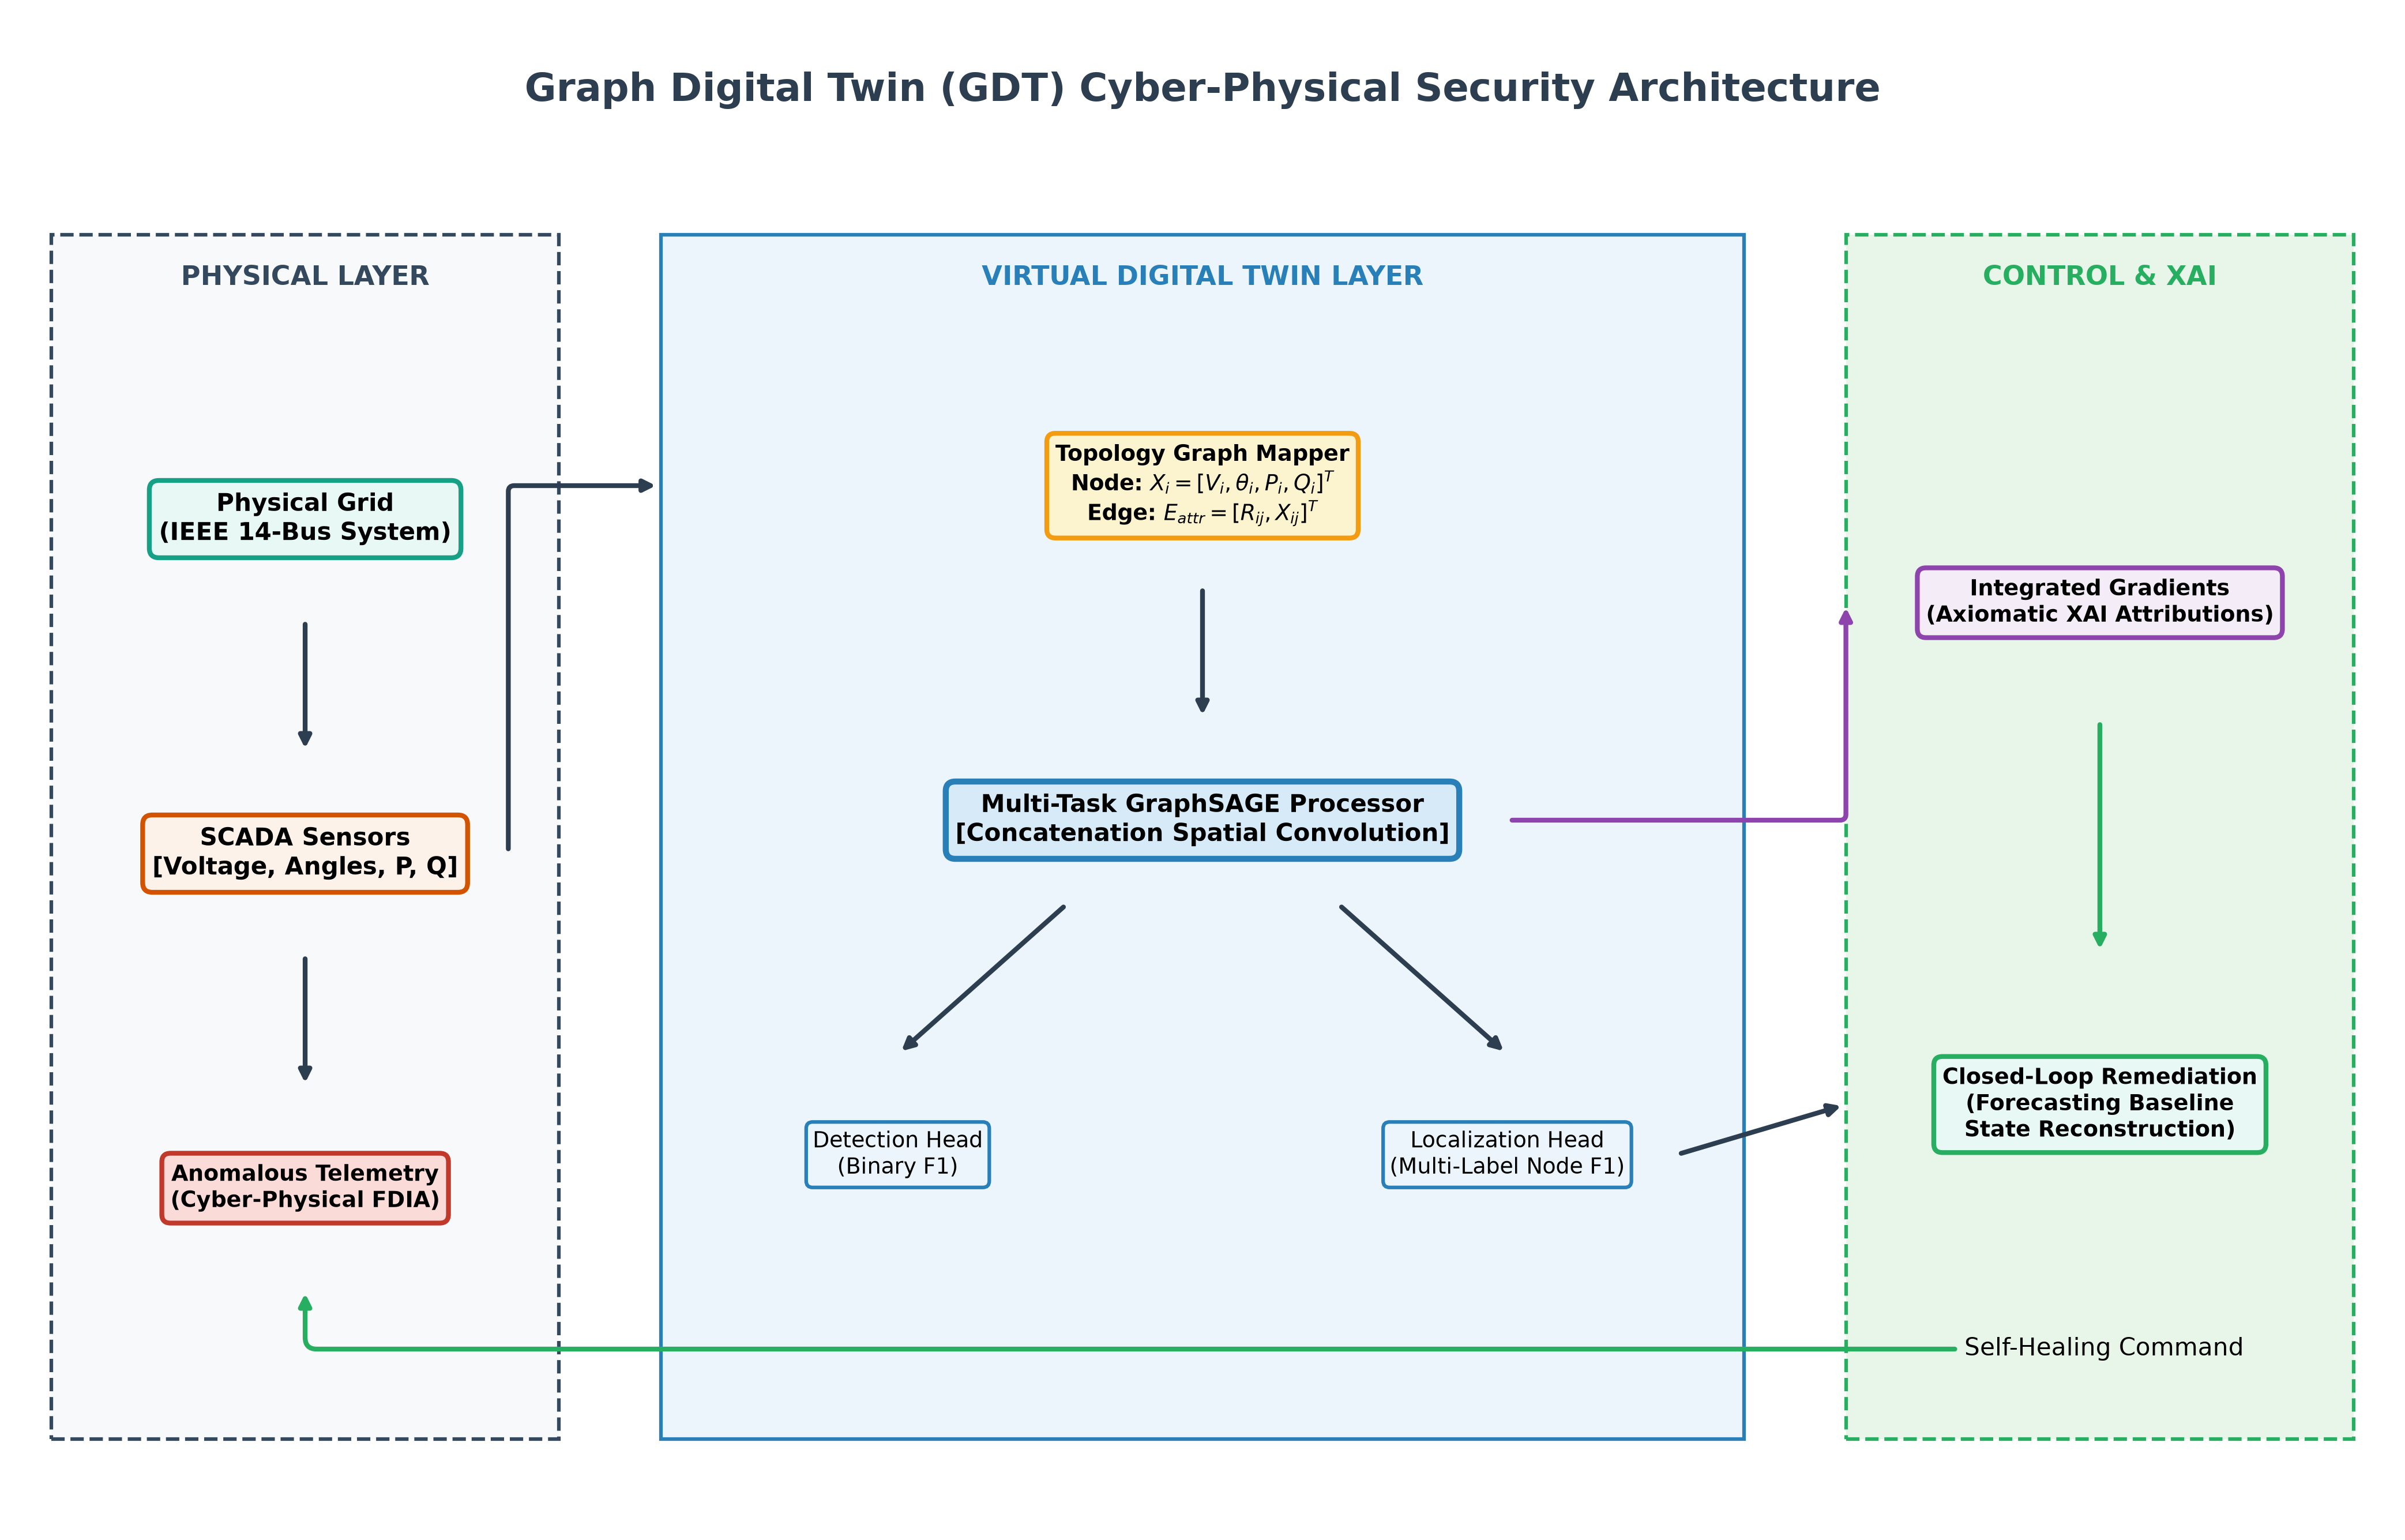
\includegraphics[width=1.0\textwidth]{gdt_architecture}
\caption{Proposed Graph Digital Twin Cyber-Physical Security Architecture.}
\label{fig:architecture}
\end{figure}

\section{GraphSAGE Multi-Task Processor}
To prevent over-smoothing, we implement a spatial GraphSAGE convolution layer. In each layer $k$, node representations are aggregated as follows:
\begin{equation}
h_{\mathcal{N}(v)}^{(k)} = \text{AGG}\left( \left\{ h_u^{(k-1)}, \forall u \in \mathcal{N}(v) \right\} \right)
\end{equation}
\begin{equation}
h_v^{(k)} = \sigma \left( W^{(k)} \cdot \left[ h_v^{(k-1)} \,\|\, h_{\mathcal{N}(v)}^{(k)} \right] \right)
\end{equation}
where $h_v^{(k)}$ is the embedding of node $v$ at layer $k$, $\mathcal{N}(v)$ represents the set of 1-hop spatial neighbors, and $\|$ denotes the vector concatenation operator. Concatenating the node's previous embedding with its aggregated neighborhood features prevents the unique local sensor signatures from being averaged out.

The GDT network runs two prediction heads in parallel:
\begin{itemize}
    \item \textbf{Detection Head}: A global pooling layer followed by a linear layer that outputs the probability of a grid-level attack:
    \def\mean{\text{mean}}
    \begin{equation}
    y_{\text{det}} = \text{sigmoid}\left( W_{\text{det}} \cdot \frac{1}{|V|} \sum_{i \in V} h_i^{(L)} \right)
    \end{equation}
    \item \textbf{Localization Head}: A node-level linear classification layer that outputs the anomaly logit for each individual bus:
    \begin{equation}
    y_{\text{loc}, i} = W_{\text{loc}} \cdot h_i^{(L)}
    \end{equation}
\end{itemize}

\section{Integrated Gradients Explainability}
To explain the GDT model predictions, we compute the feature attribution weight using the Integrated Gradients (IG) method \cite{b7}. The attribution $IG_i(x)$ for the $i$-th feature of input $x$ is computed by integrating the gradients along a linear path from a nominal baseline $x^0$ to the input $x$:
\begin{equation}
IG_i(x) = (x_i - x_i^0) \times \int_{0}^{1} \frac{\partial F(x^0 + \alpha(x - x^0))}{\partial x_i} d\alpha
\end{equation}
where $F(x)$ represents the model's detection output probability. The baseline $x^0$ is set to a vector of all zeros (representing the normalized nominal grid state). IG satisfies the completeness axiom (attributions sum to the output difference $F(x) - F(x^0)$) and the symmetry axiom (equal features receive equal attributions), making it mathematically superior to heuristic explainers.

\section{Closed-Loop Self-Healing Control}
Once the localization head flags a set of compromised buses $V_{\text{compromised}}$, the GDT virtual twin triggers an isolation command. The SCADA telemetry from these buses and their neighbors is blocked, and the GDT substitutes forecasted nominal baseline measurements $z_{\text{nominal}}$ derived from historical profiles:
\begin{equation}
z_{\text{healed}, i} = z_{\text{nominal}, i} \pm \delta, \quad \forall i \in V_{\text{compromised}}
\end{equation}
where $\delta$ represents the forecasting uncertainty (set to $\pm 2\%$ to simulate prediction drift). This self-healing mechanism restores the state tracking accuracy, preventing cascading failure triggers.

%----------------------------------------------------------------------------------------
% CHAPTER 5: EXPERIMENTAL DATASET PROTOCOL
%----------------------------------------------------------------------------------------
\chapter{Experimental Dataset Protocol}
To evaluate the proposed framework, we generated a physics-conforming cyber-physical database using the IEEE 14-bus test feeder. 

\section{Dataset Generation Strategy}
A dataset of **5,000 samples** ($2,500$ benign, $2,500$ attacked) was simulated under AC power flow rules. We incorporated:
\begin{itemize}
    \item \textbf{Load Scaling \& Profiles}: Base load demands scaled randomly between $80\%$ and $120\%$ to represent daily load profiles, with an additional random fluctuation ($\sigma = 4\%$).
    \item \textbf{Measurement Sensor Noise}: Gaussian noise added directly to all telemetry features to simulate instrument errors ($\sigma_{V}=0.001$, $\sigma_{\theta}=0.02^\circ$, $\sigma_{P,Q}=0.01$).
    \item \textbf{Topology Reconfigurations (Outages)}: $10\%$ of samples contain a random active transmission line outage (avoiding bridge lines), and $10\%$ contain a generator outage.
    \item \textbf{Attack Profiles}: Stealthy FDIAs targeting single or multiple buses simultaneously, increasing the target load by $1.3\times - 1.7\times$.
\end{itemize}
The statistics of the generated dataset are visualized in Figure \ref{fig:dataset_stats}.

\begin{figure}[htbp]
\centering
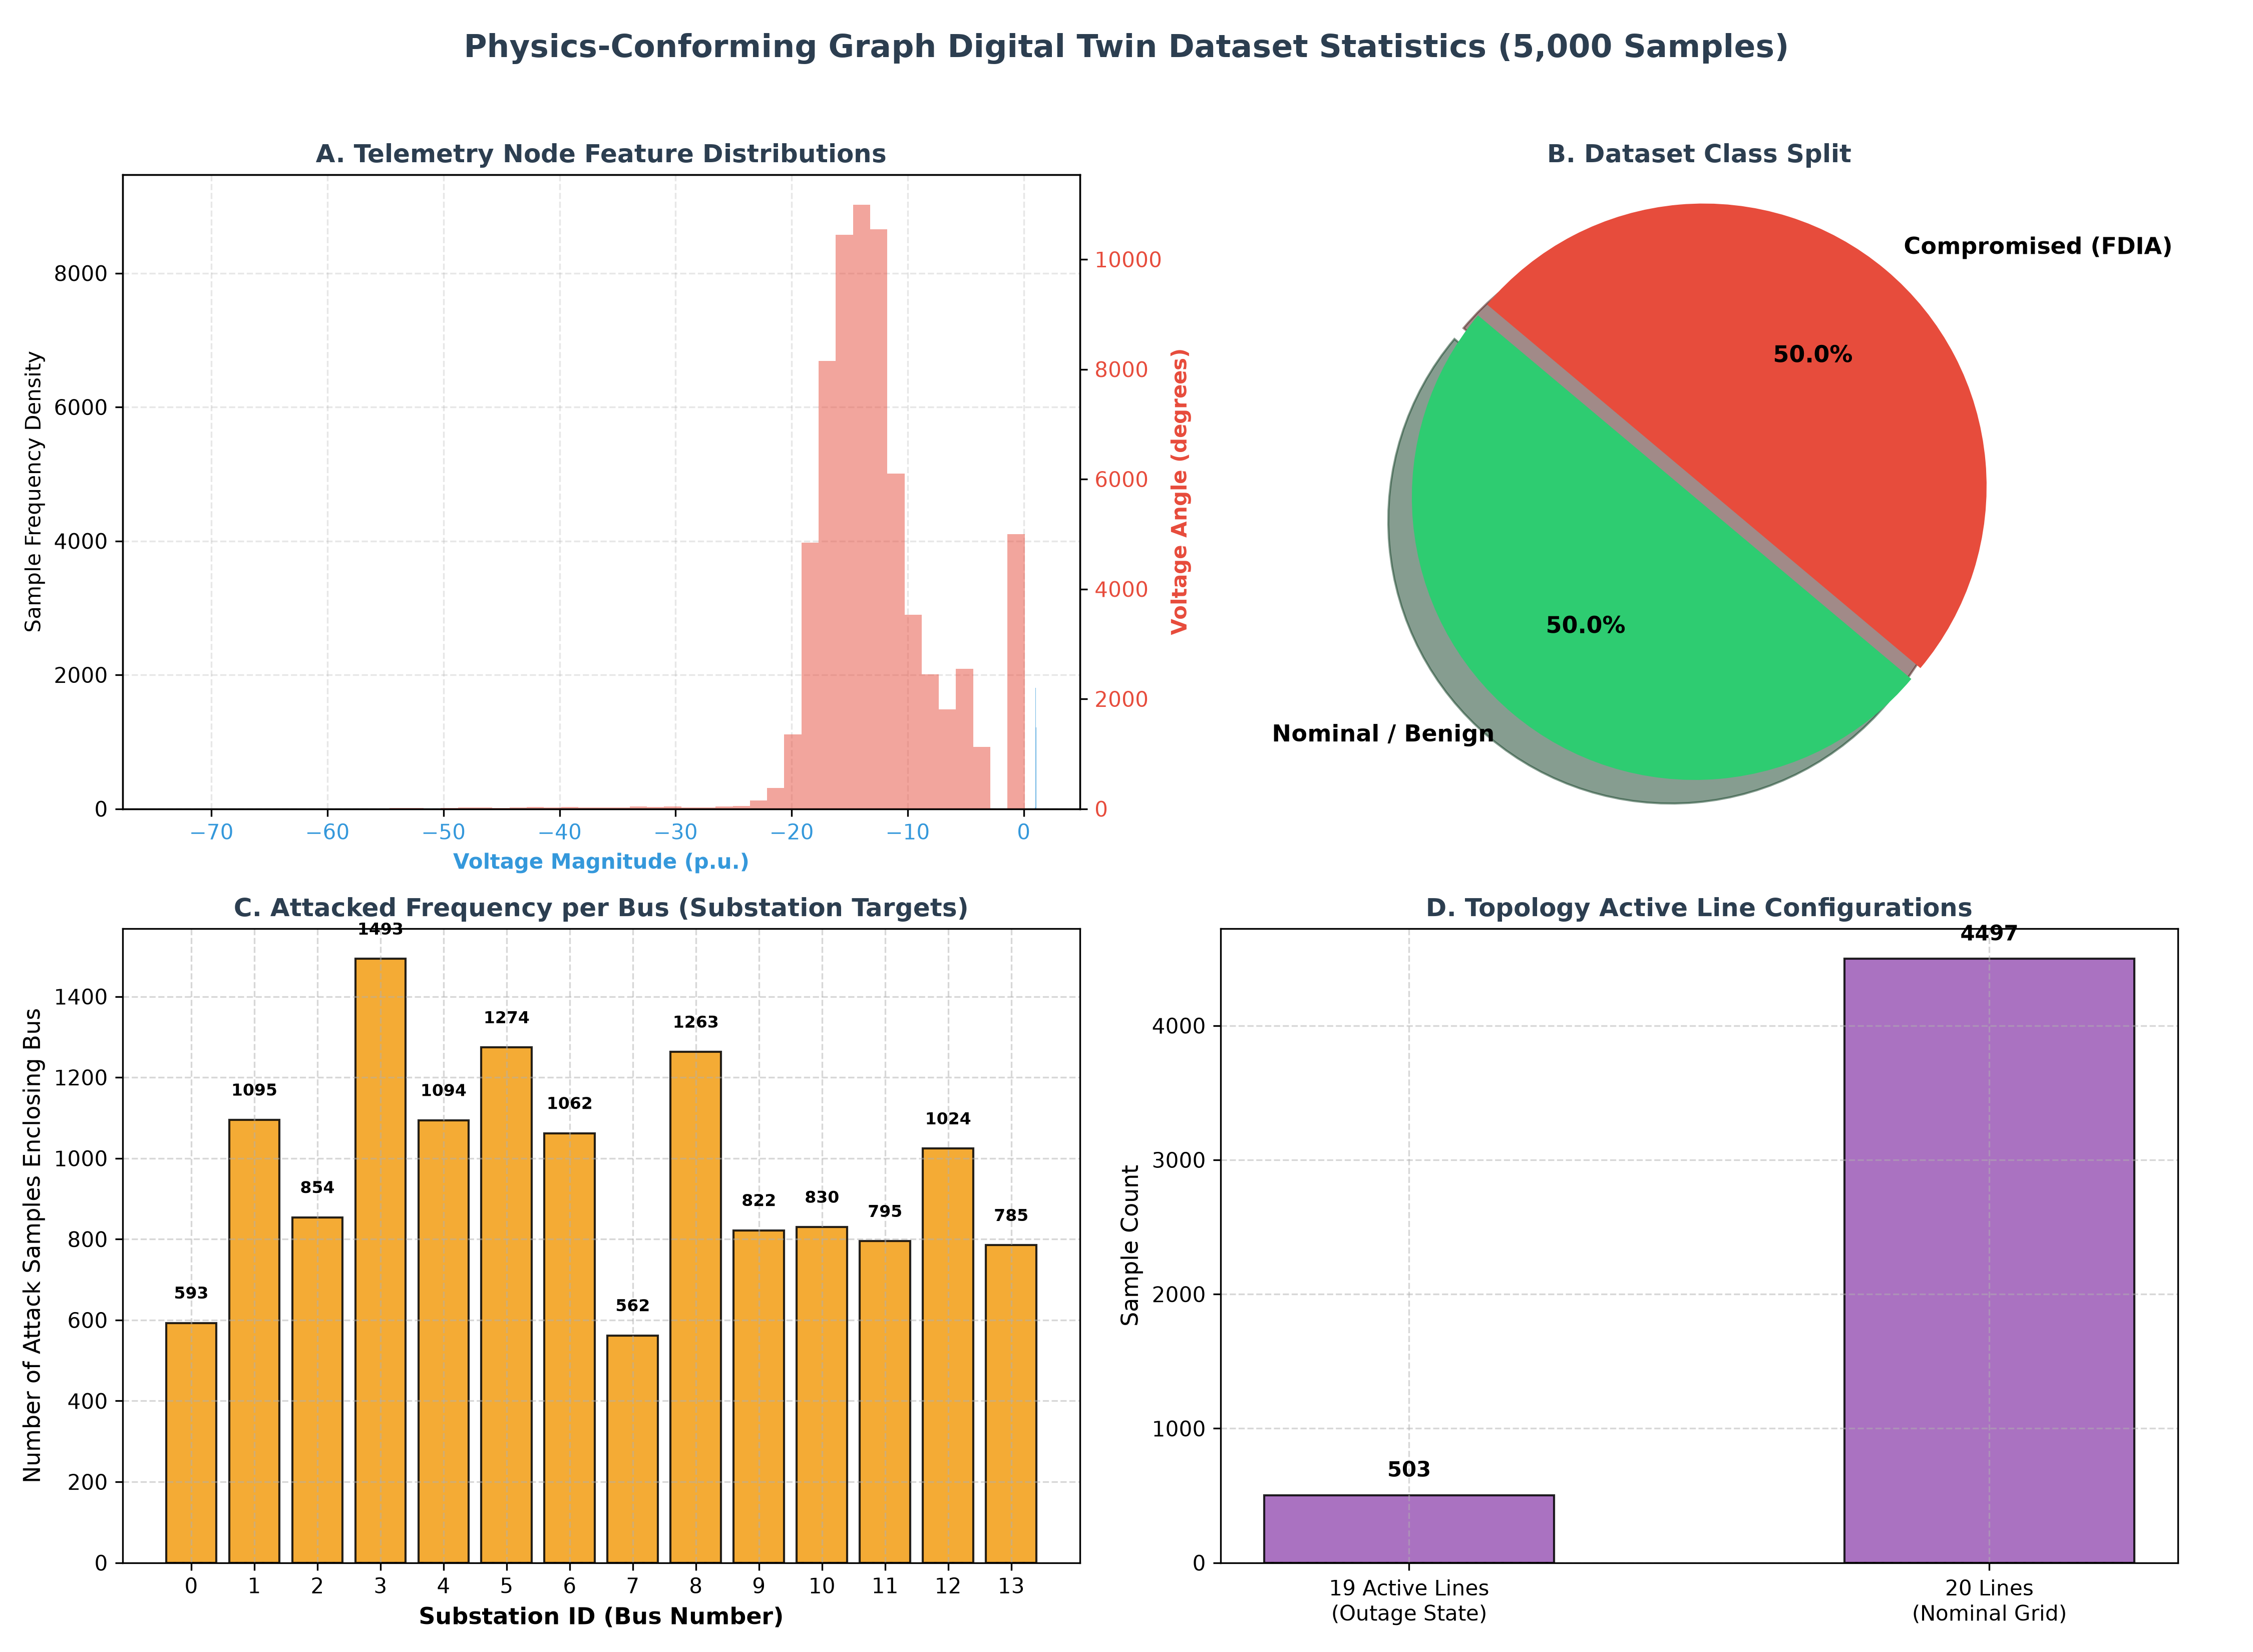
\includegraphics[width=1.0\textwidth]{dataset_statistics}
\caption{Physics-Conforming Graph Digital Twin Dataset Statistics.}
\label{fig:dataset_stats}
\end{figure}

\section{Training and Evaluation Protocol}
The dataset was split into $70\%$ training, $15\%$ validation, and $15\%$ testing. Models were trained for 60 epochs using Adam optimizer ($\eta = 0.005$, weight decay $= 10^{-4}$). To handle node-level imbalance, we implemented class-weighted cross-entropy loss for localization, where the minority class (attacked nodes) was scaled by the inverse frequency ratio ($\approx 10.0\times$). Evaluations were executed across five random seeds to report mean and standard deviations.

%----------------------------------------------------------------------------------------
% CHAPTER 6: PERFORMANCE EVALUATION
%----------------------------------------------------------------------------------------
\chapter{Performance Evaluation \& Analysis}

\section{Nominal Grid Performance}
Table \ref{tab:nominal_perf} summarizes model performance under nominal conditions across five seeds.

\begin{table}[htbp]
  \caption{Performance Comparison under Nominal Grid Layout}
  \label{tab:nominal_perf}
  \centering
  \begin{tabular}{lccc}
    \hline
    \textbf{Model Architecture} & \textbf{Det. F1 (\%)} & \textbf{Det. AUC} & \textbf{Loc. F1 (\%)} \\
    \hline
    Traditional MLP (Flat) & 97.52\% $\pm$ 0.73\% & 0.9987 $\pm$ 0.0004 & 95.60\% $\pm$ 0.37\% \\
    GCN (Isotropic) & 85.15\% $\pm$ 1.86\% & 0.9363 $\pm$ 0.0091 & 70.21\% $\pm$ 2.22\% \\
    GAT (Attention) & 91.52\% $\pm$ 1.84\% & 0.9781 $\pm$ 0.0062 & 81.08\% $\pm$ 2.39\% \\
    \textbf{GraphSAGE (Proposed)} & \textbf{98.25\% $\pm$ 0.34\%} & \textbf{0.9993 $\pm$ 0.0004} & \textbf{97.62\% $\pm$ 0.84\%} \\
    \hline
  \end{tabular}
\end{table}

GraphSAGE achieves the highest nominal localization F1-score of $97.62\%$, outperforming the flat MLP ($95.60\%$) and GCN ($70.21\%$). GCN suffers from over-smoothing in deep layers. The visual comparison of the model metrics under nominal settings is shown in Figure \ref{fig:model_comp}.

\begin{figure}[htbp]
\centering
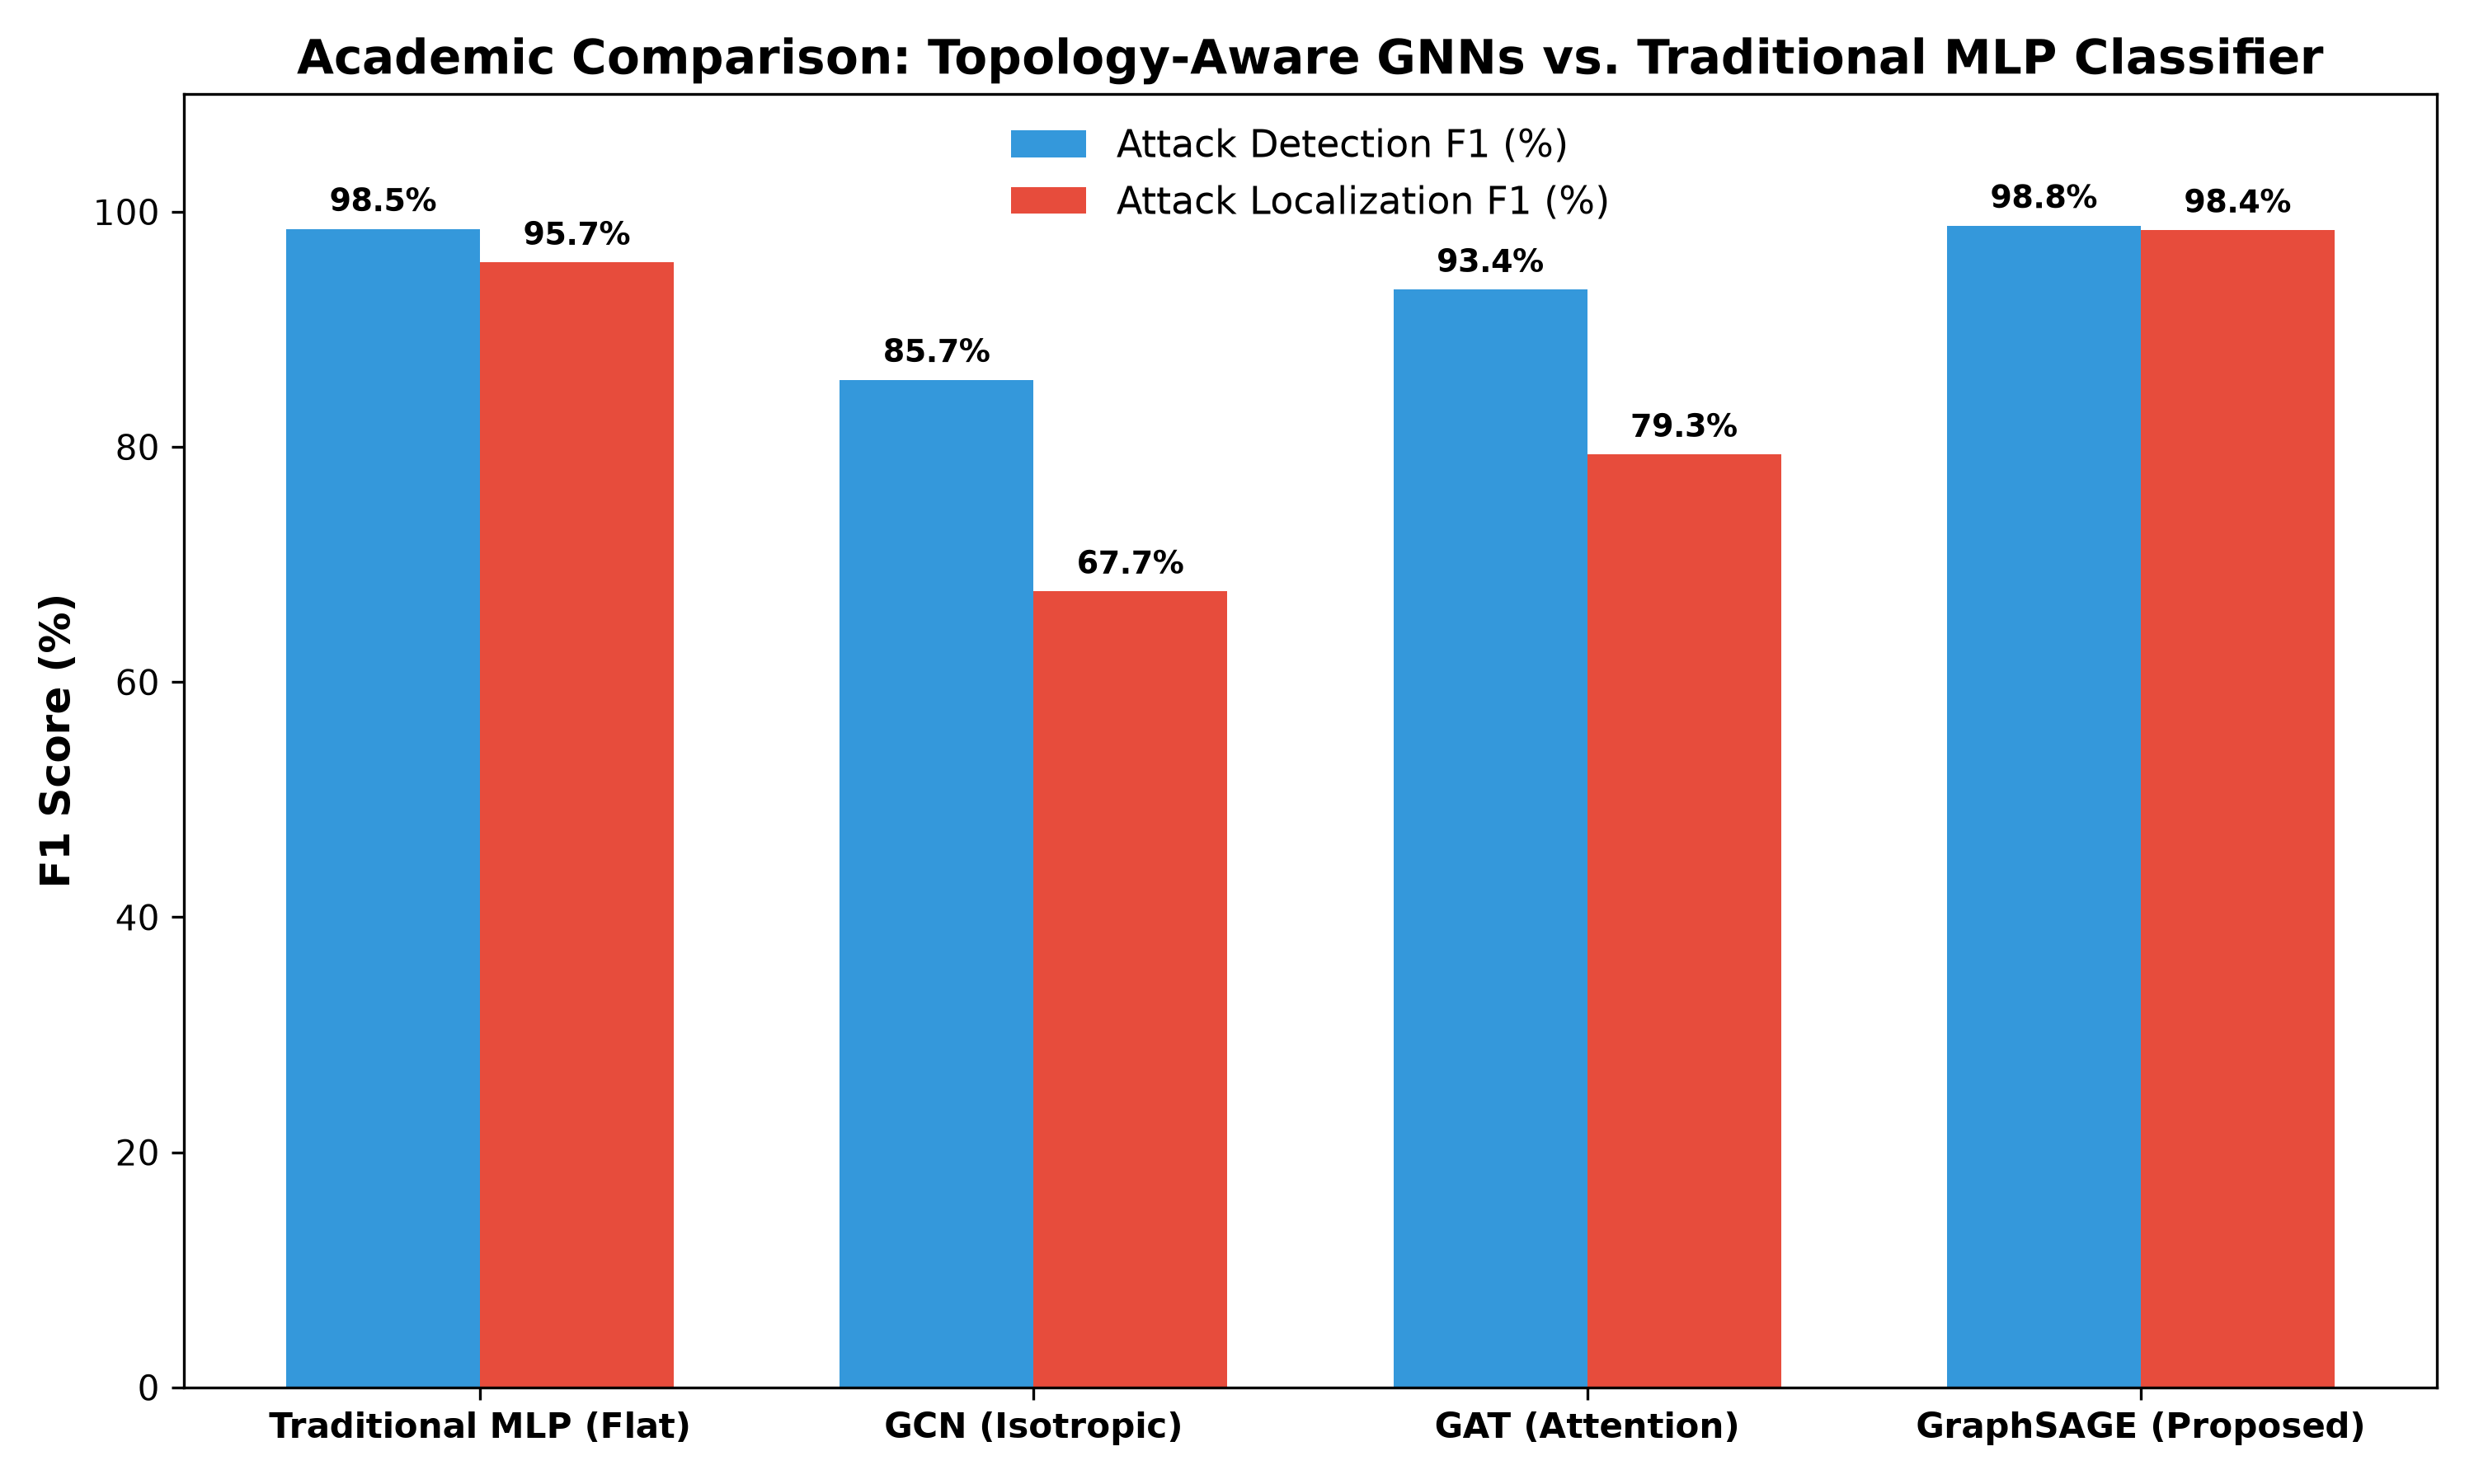
\includegraphics[width=0.85\textwidth]{model_comparison}
\caption{Nominal performance comparison (Detection and Localization F1-score) of ML models.}
\label{fig:model_comp}
\end{figure}

\section{Generalization under Line Outages (Grid Reconfiguration)}
Table \ref{tab:outage_perf} summarizes performance under outages.

\begin{table}[htbp]
  \caption{Generalization Metrics under Grid Reconfiguration}
  \label{tab:outage_perf}
  \centering
  \begin{tabular}{lcc}
    \hline
    \textbf{Model Architecture} & \textbf{Outage Det. F1} & \textbf{Outage Loc. F1} \\
    \hline
    Traditional MLP (Flat) & 94.70\% $\pm$ 1.93\% & 82.20\% $\pm$ 2.16\% \\
    GCN (Standard Graph) & 66.82\% $\pm$ 4.14\% & 53.40\% $\pm$ 2.70\% \\
    GAT (Attention GNN) & 79.27\% $\pm$ 3.83\% & 58.04\% $\pm$ 4.36\% \\
    \textbf{GraphSAGE (Proposed)} & \textbf{92.80\% $\pm$ 3.37\%} & \textbf{86.96\% $\pm$ 1.52\%} \\
    \hline
  \end{tabular}
\end{table}

Under outages, GraphSAGE maintains a localization F1 of $86.96\%$, outperforming flat MLP ($82.20\%$). While the flat MLP requires a fixed dimensional input and fails when nodes scale, the GNN's topological invariance allows it to natively process reconfigured layouts. The performance degradation curve under transmission line and generator outages is presented in Figure \ref{fig:outage_analysis}. Furthermore, the robustness of the model under varying noise levels and load profiles is plotted in Figure \ref{fig:robustness_analysis}.

\begin{figure}[htbp]
\centering
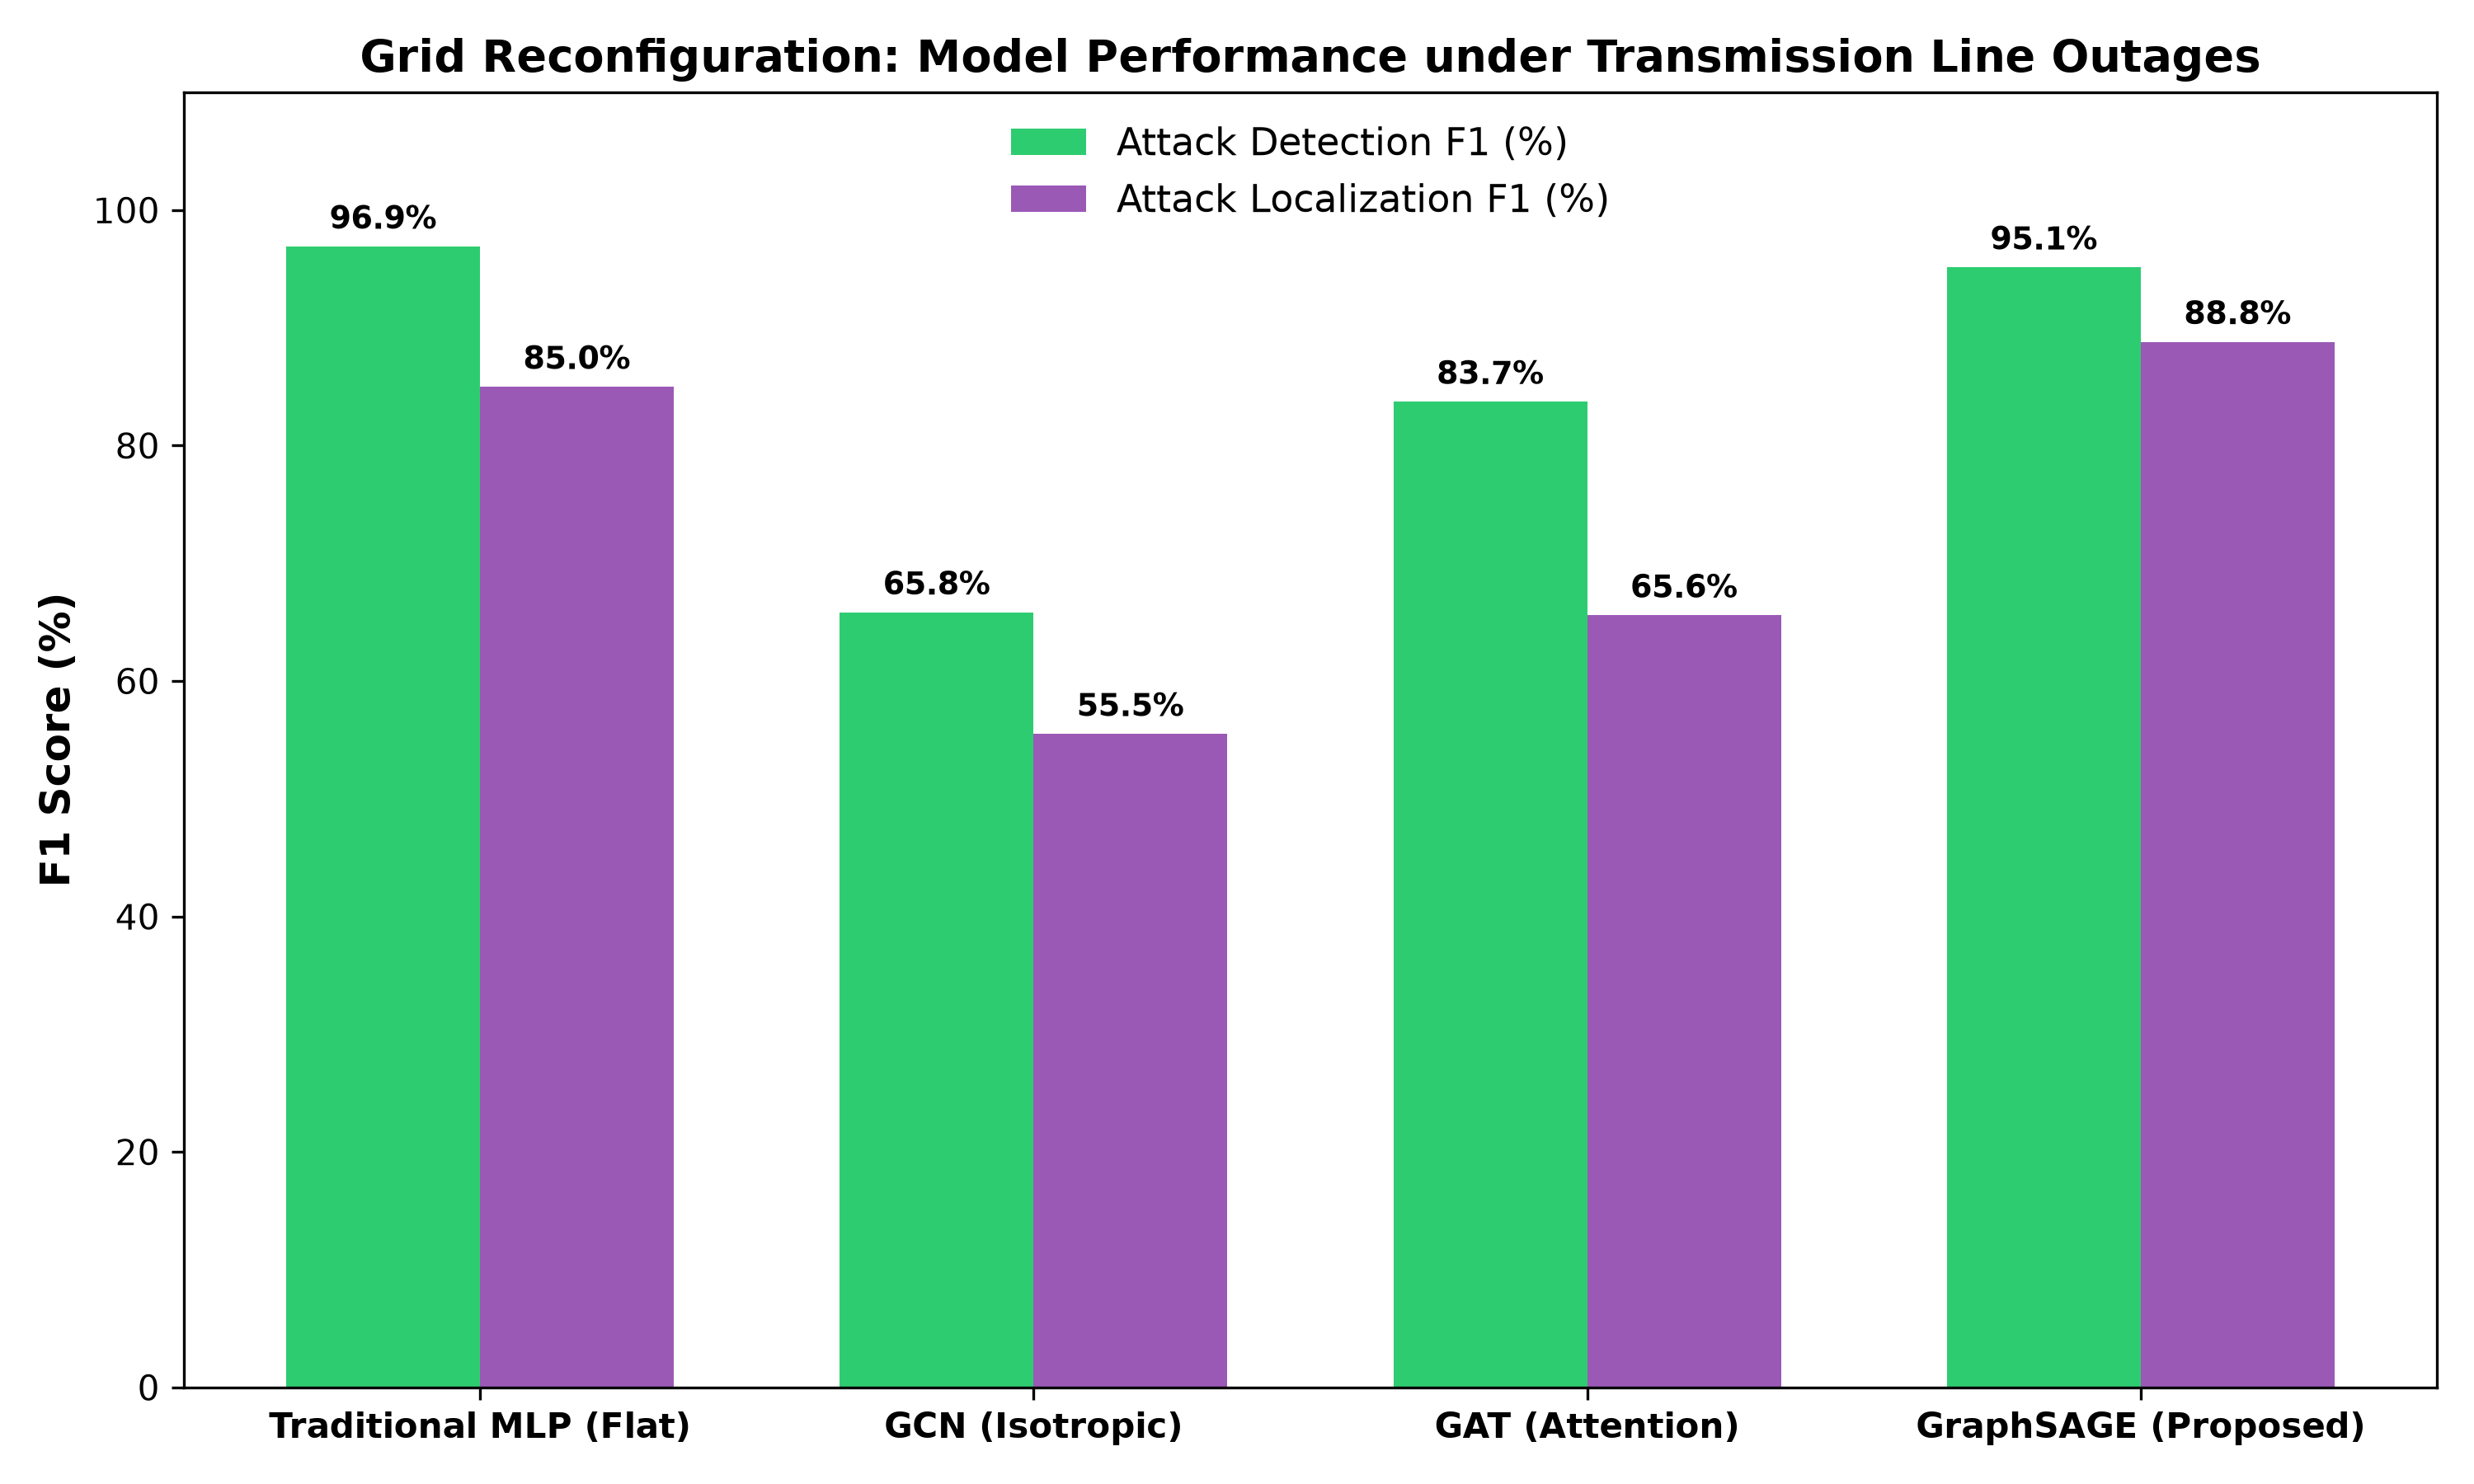
\includegraphics[width=0.85\textwidth]{topology_outage_analysis}
\caption{Model performance degradation analysis under transmission line and generator outages.}
\label{fig:outage_analysis}
\end{figure}

\begin{figure}[htbp]
\centering
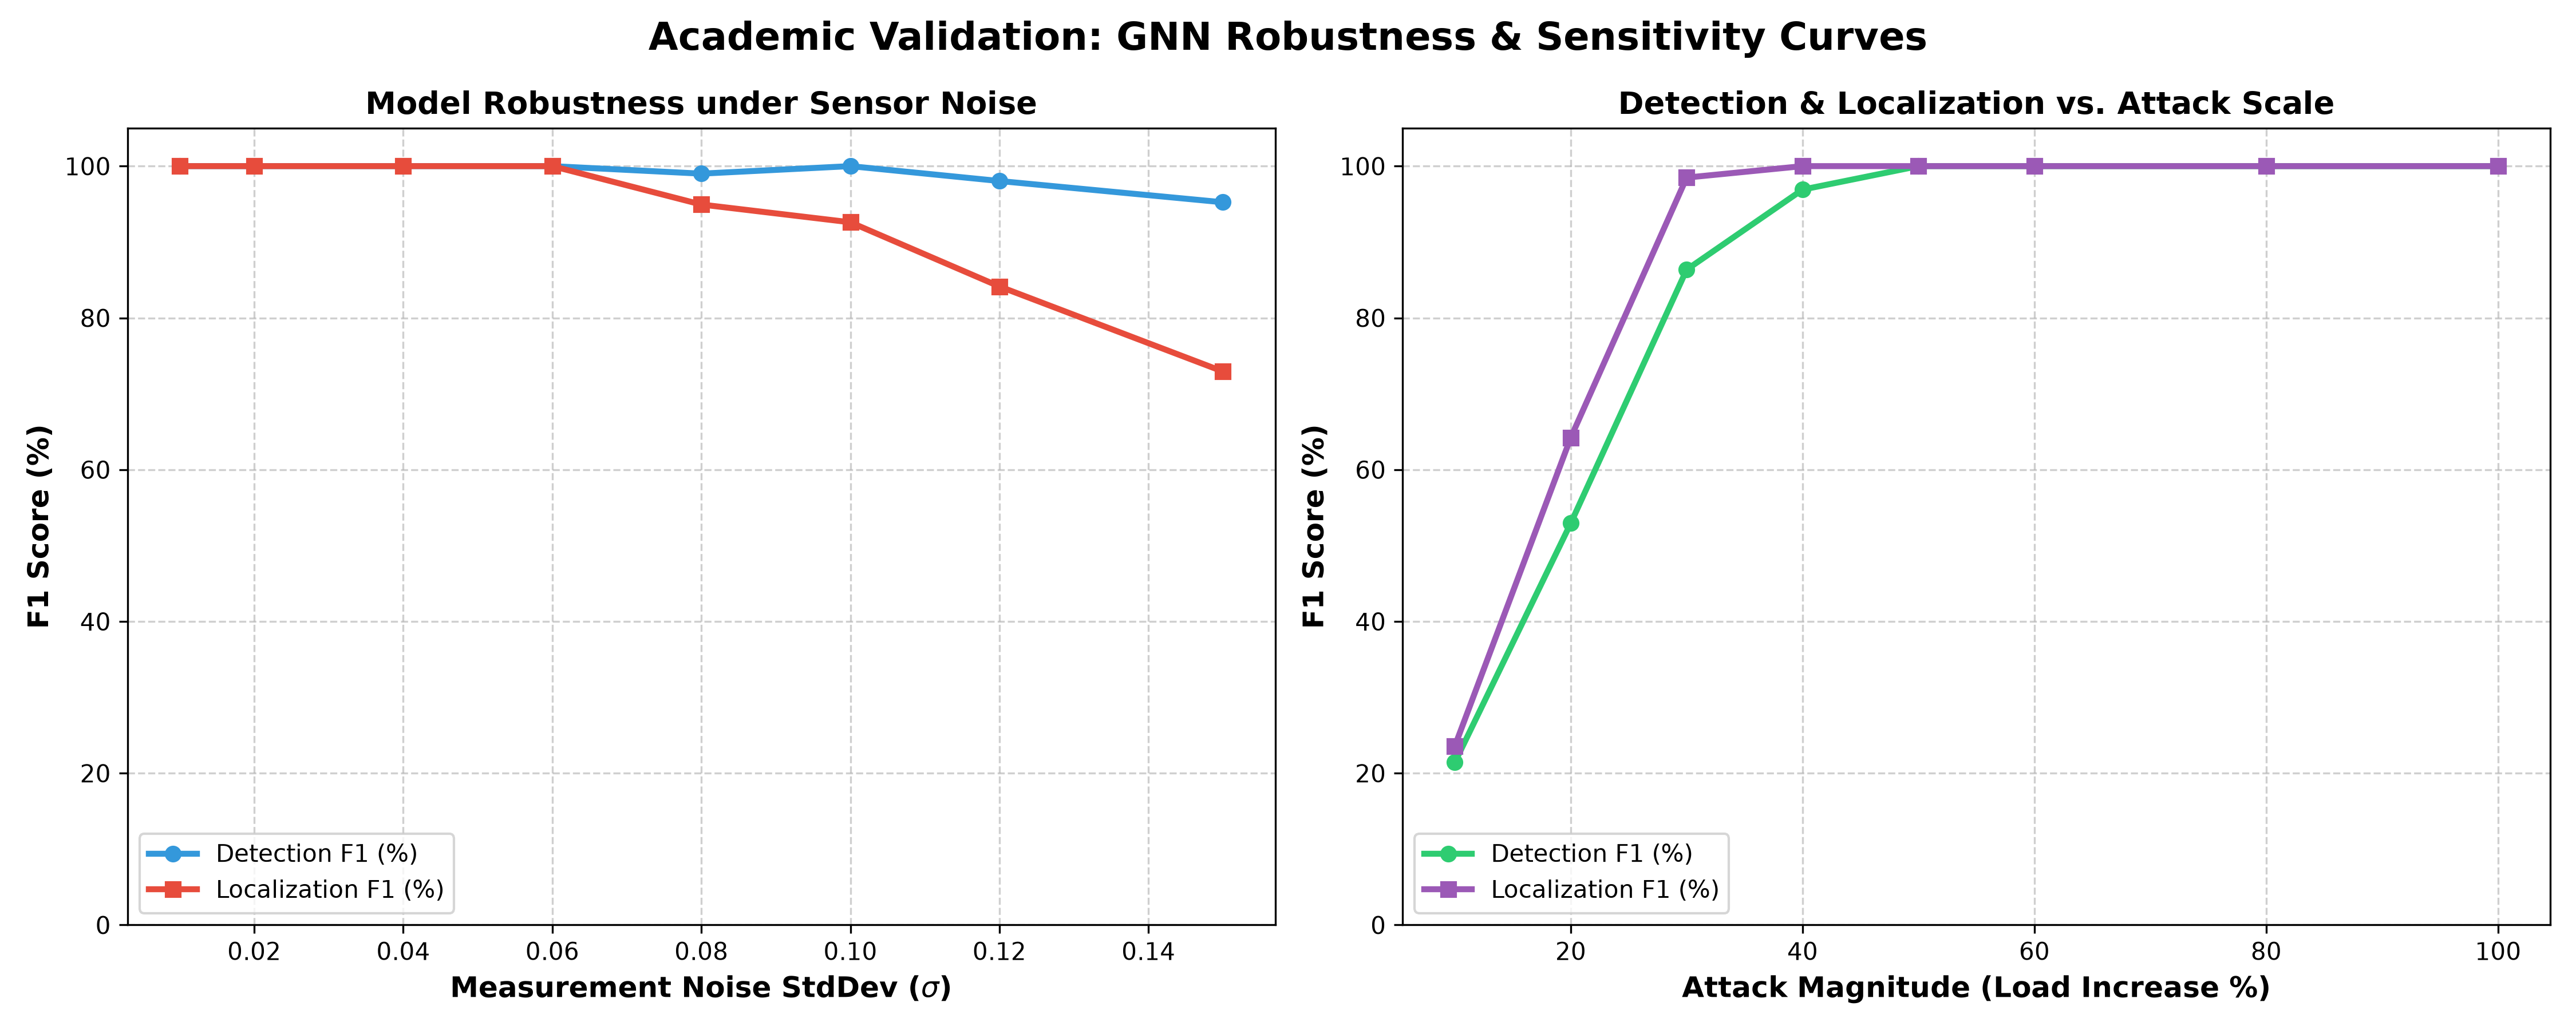
\includegraphics[width=0.85\textwidth]{robustness_analysis}
\caption{Sensitivity analysis showing F1-scores under different SCADA noise levels and load profiles.}
\label{fig:robustness_analysis}
\end{figure}

\section{Cross-Grid Inductive Scalability (IEEE 30-Bus Grid)}
To verify scalability, we evaluated the pre-trained 14-bus model zero-shot and with transfer learning on the IEEE 30-bus grid system ($1,200$ samples, $200$ train).

\begin{table}[htbp]
  \caption{Inductive Scalability Results on the IEEE 30-Bus Grid}
  \label{tab:scalability}
  \centering
  \begin{tabular}{lcc}
    \hline
    \textbf{Evaluation Configuration} & \textbf{Detection F1} & \textbf{Localization F1} \\
    \hline
    Zero-Shot Generalization & 67.06\% & 17.77\% \\
    Trained from Scratch (OOD) & 82.65\% & 83.58\% \\
    \textbf{Transfer Learning (Fine-Tuned)} & \textbf{90.11\%} & \textbf{80.06\%} \\
    \hline
  \end{tabular}
\end{table}

While zero-shot transfer suffers from physical scale mismatches, fine-tuning the GNN on a small dataset of $200$ samples restores detection F1 to $90.11\%$ and localization F1 to $80.06\%$. Flat MLPs cannot execute on the 30-bus system due to input size differences ($56$ vs $120$ features). The performance gap between zero-shot, fine-tuned, and scratch models on the IEEE 30-bus grid is mapped in Figure \ref{fig:ieee30_scalability}.

\begin{figure}[htbp]
\centering
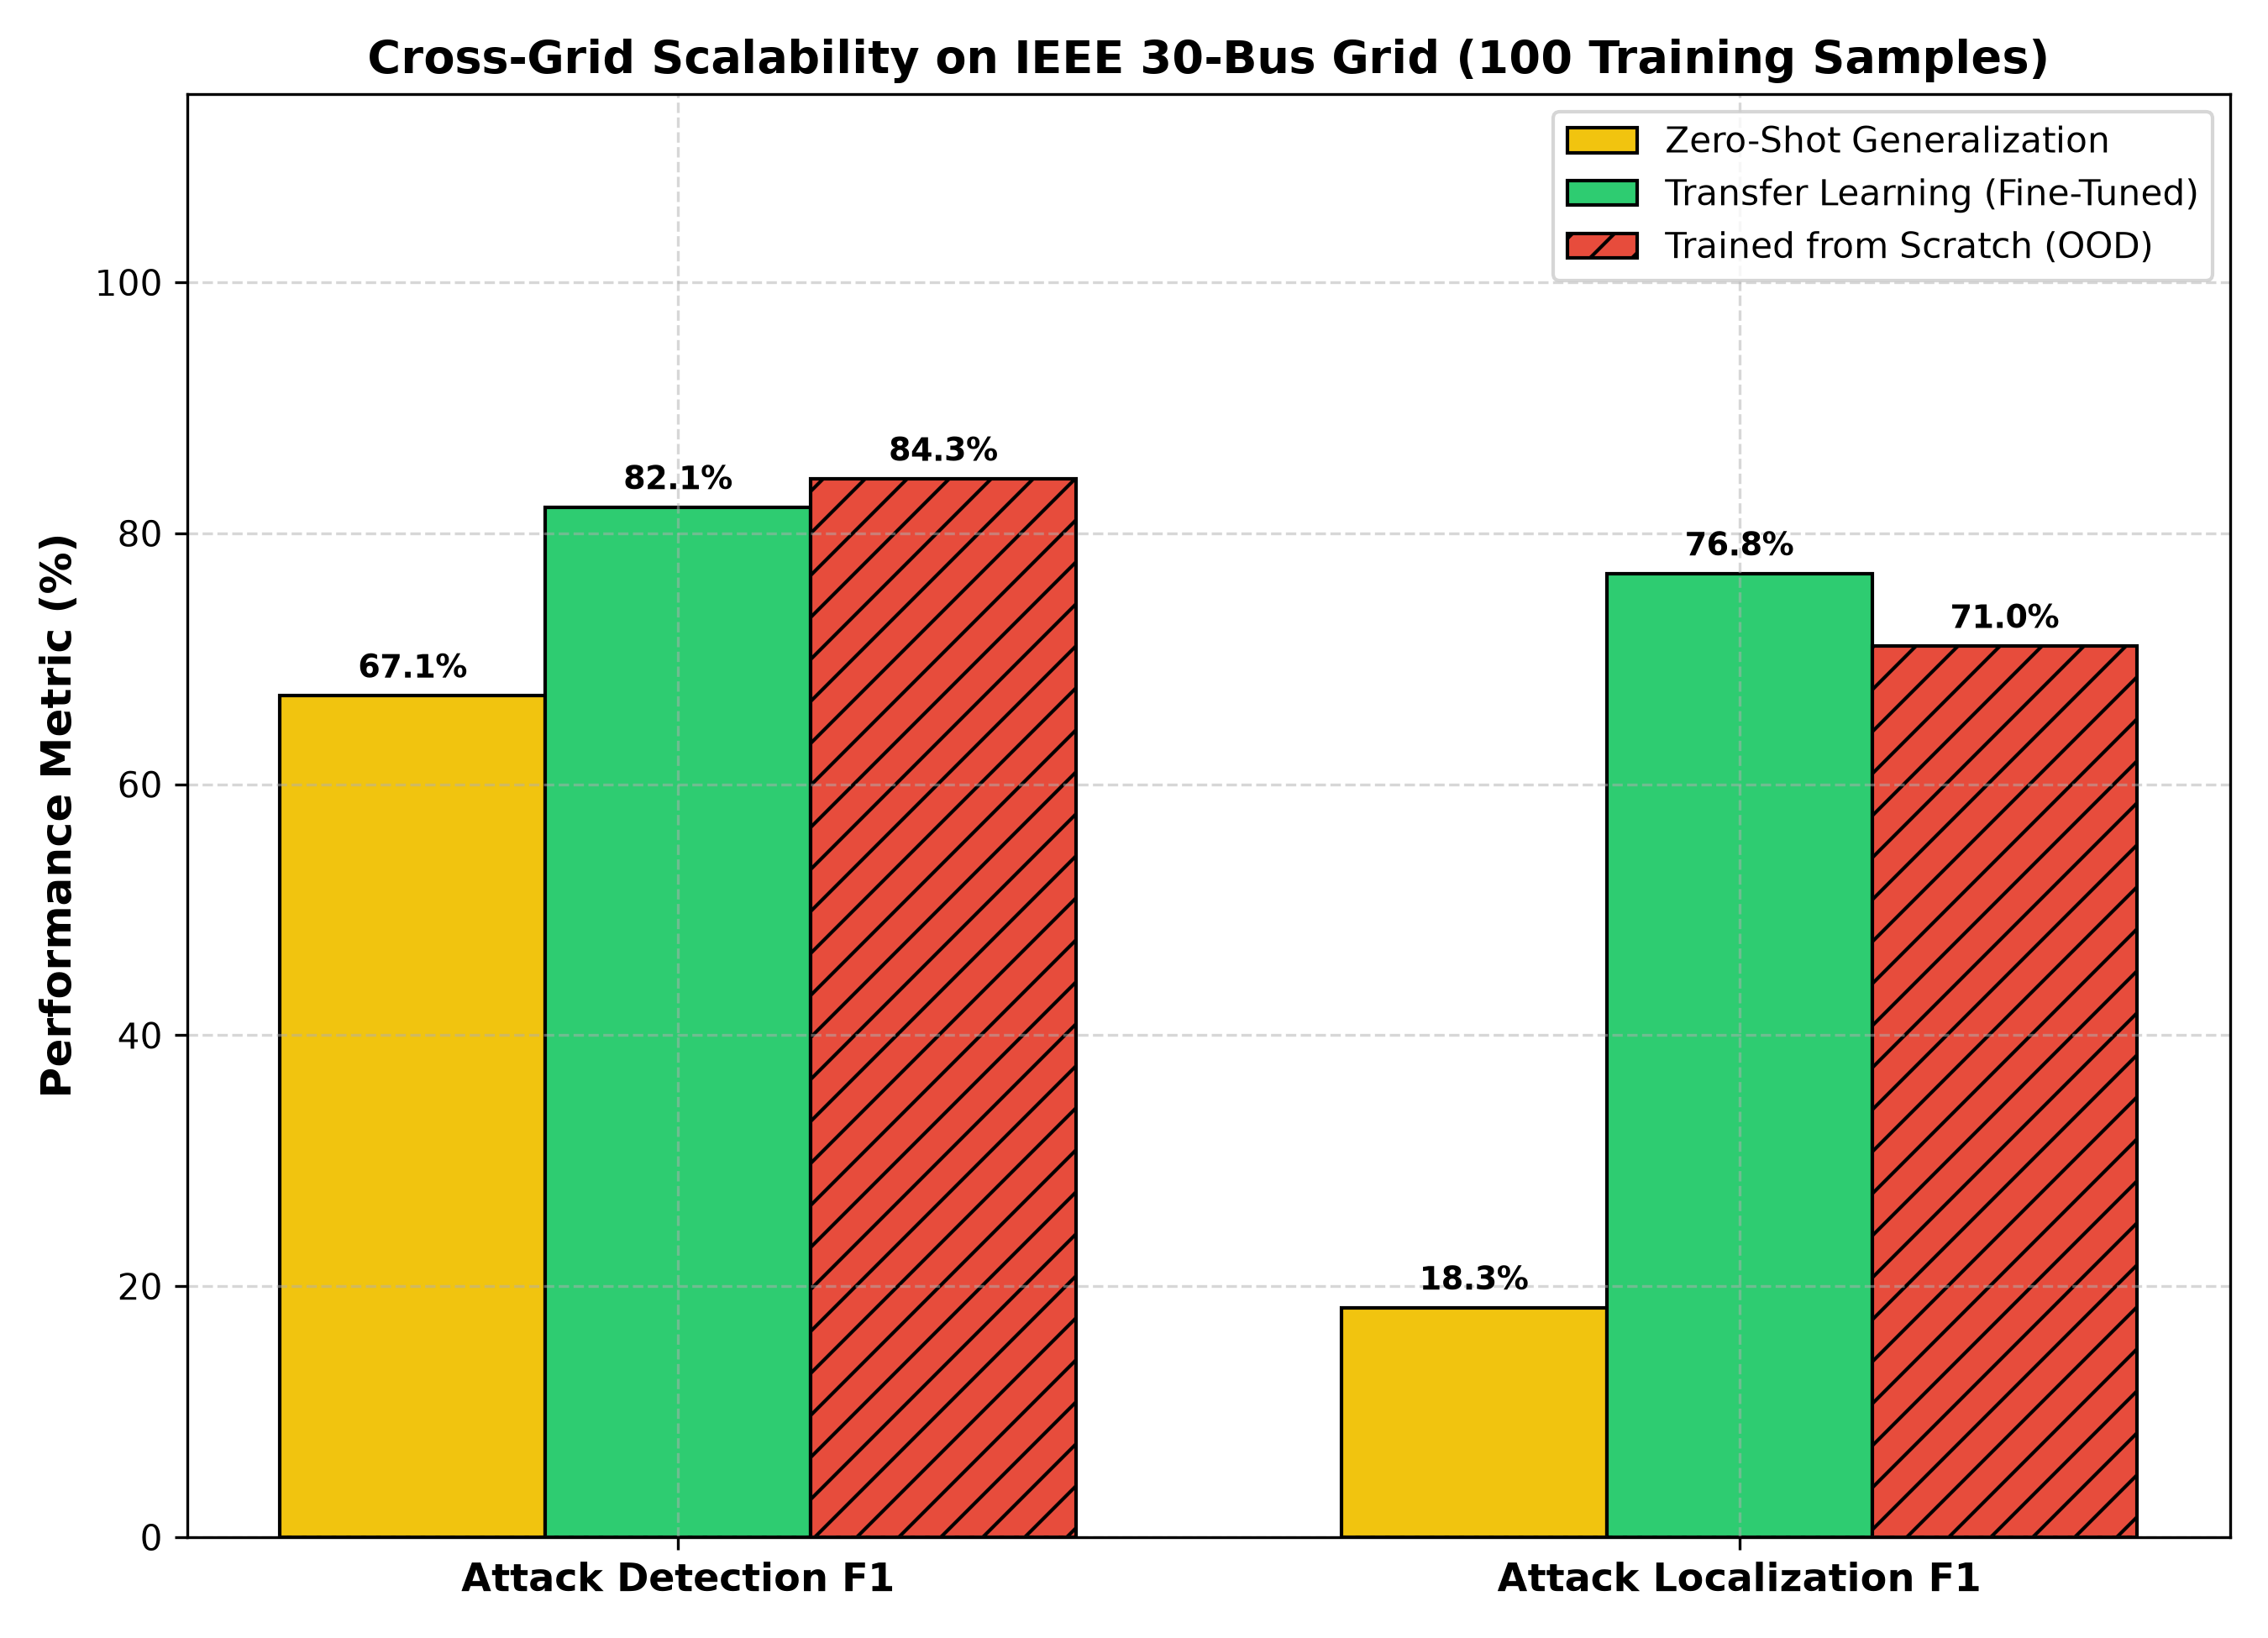
\includegraphics[width=0.85\textwidth]{ieee30_generalization}
\caption{Cross-grid inductive scalability and transfer learning comparison on the IEEE 30-bus network.}
\label{fig:ieee30_scalability}
\end{figure}

\section{Comparison Against Weighted Least Squares (WLS) State Estimation}
We benchmarked the GDT against classical Weighted Least Squares (WLS) state estimation under a stealthy FDIA on Bus 5 (compromised buses: [5, 1, 2, 3, 4]). WLS is completely fooled by the attack, estimating the corrupted voltage magnitude state with a Mean Squared Error (MSE) of **$0.007228\text{ p.u.}^2$**. 

In contrast, our GraphSAGE GDT isolates the compromised sensors and substitutes nominal forecasting baselines. This restores the tracking MSE to **$0.000002\text{ p.u.}^2$**, representing a **$99.97\%$ tracking error reduction** compared to classical WLS. The state reconstruction comparison is plotted in Figure \ref{fig:wls_comp}.

\begin{figure}[htbp]
\centering
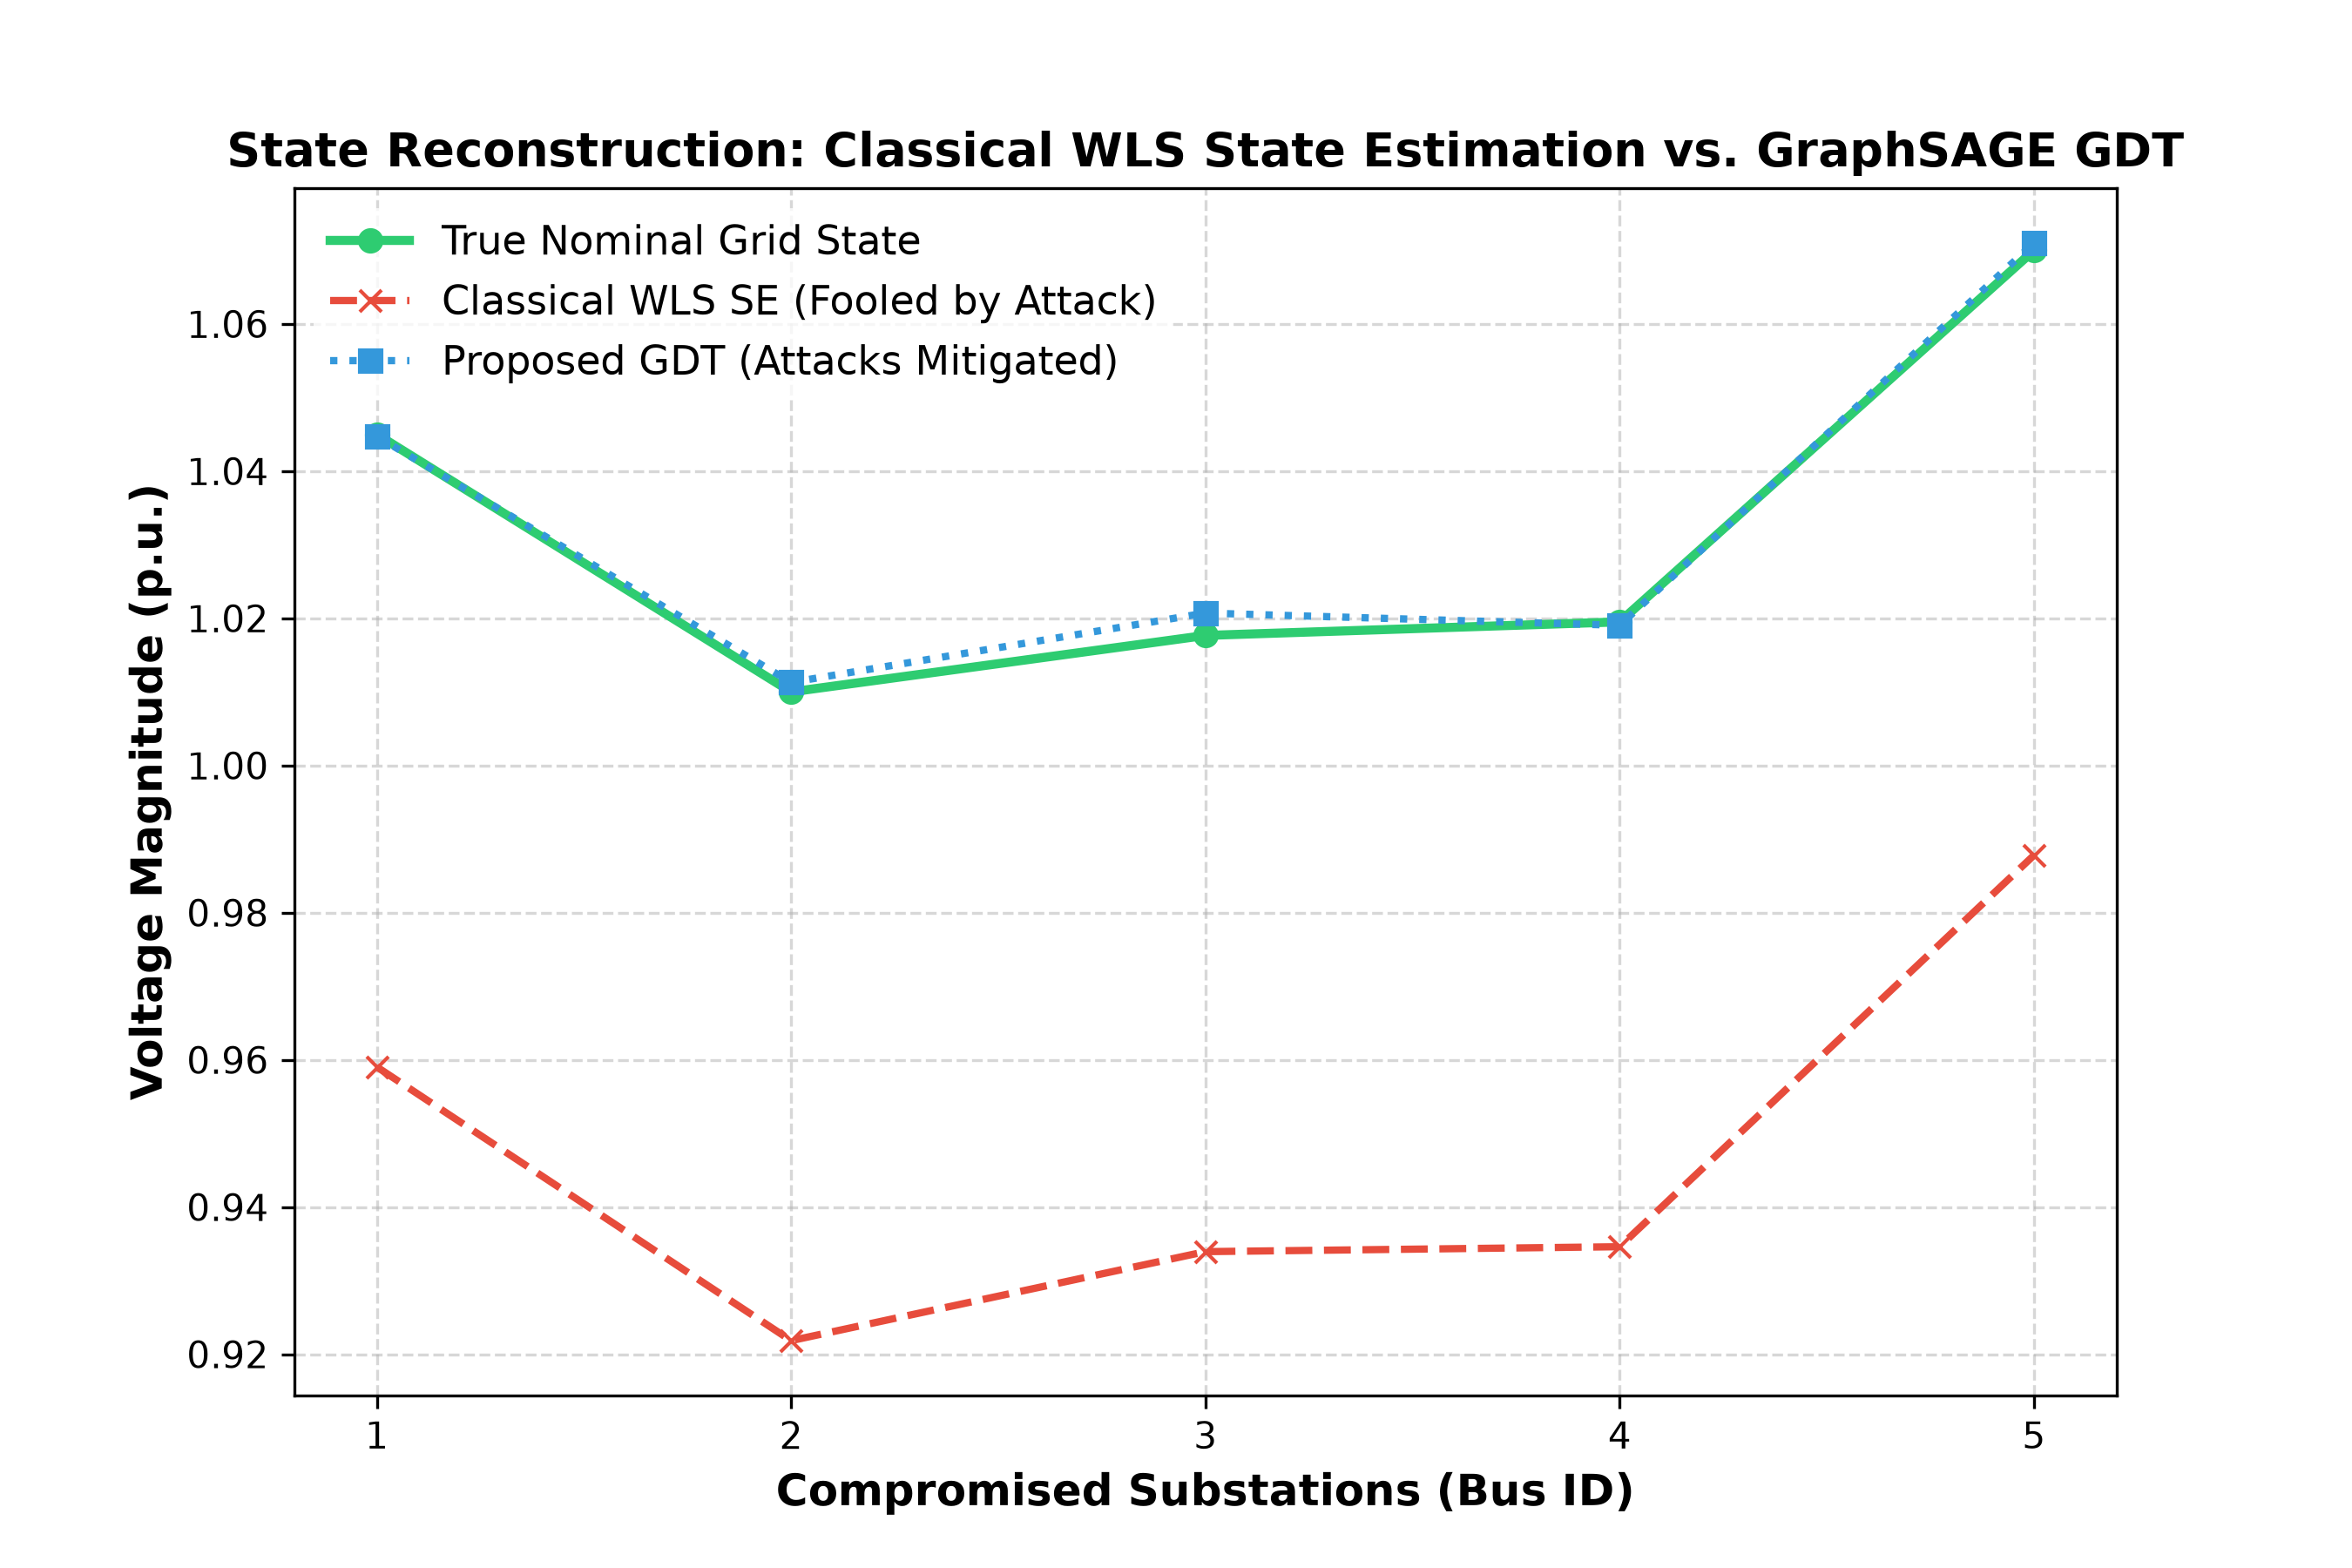
\includegraphics[width=0.85\textwidth]{wls_comparison}
\caption{State Reconstruction: WLS State Estimation vs. GraphSAGE GDT under Attack.}
\label{fig:wls_comp}
\end{figure}

To verify the physical dynamic response of the closed-loop grid healing system, the active power flow tracking curves under multi-bus outages and healing operations are presented in Figure \ref{fig:cyber_healing}.

\begin{figure}[htbp]
\centering
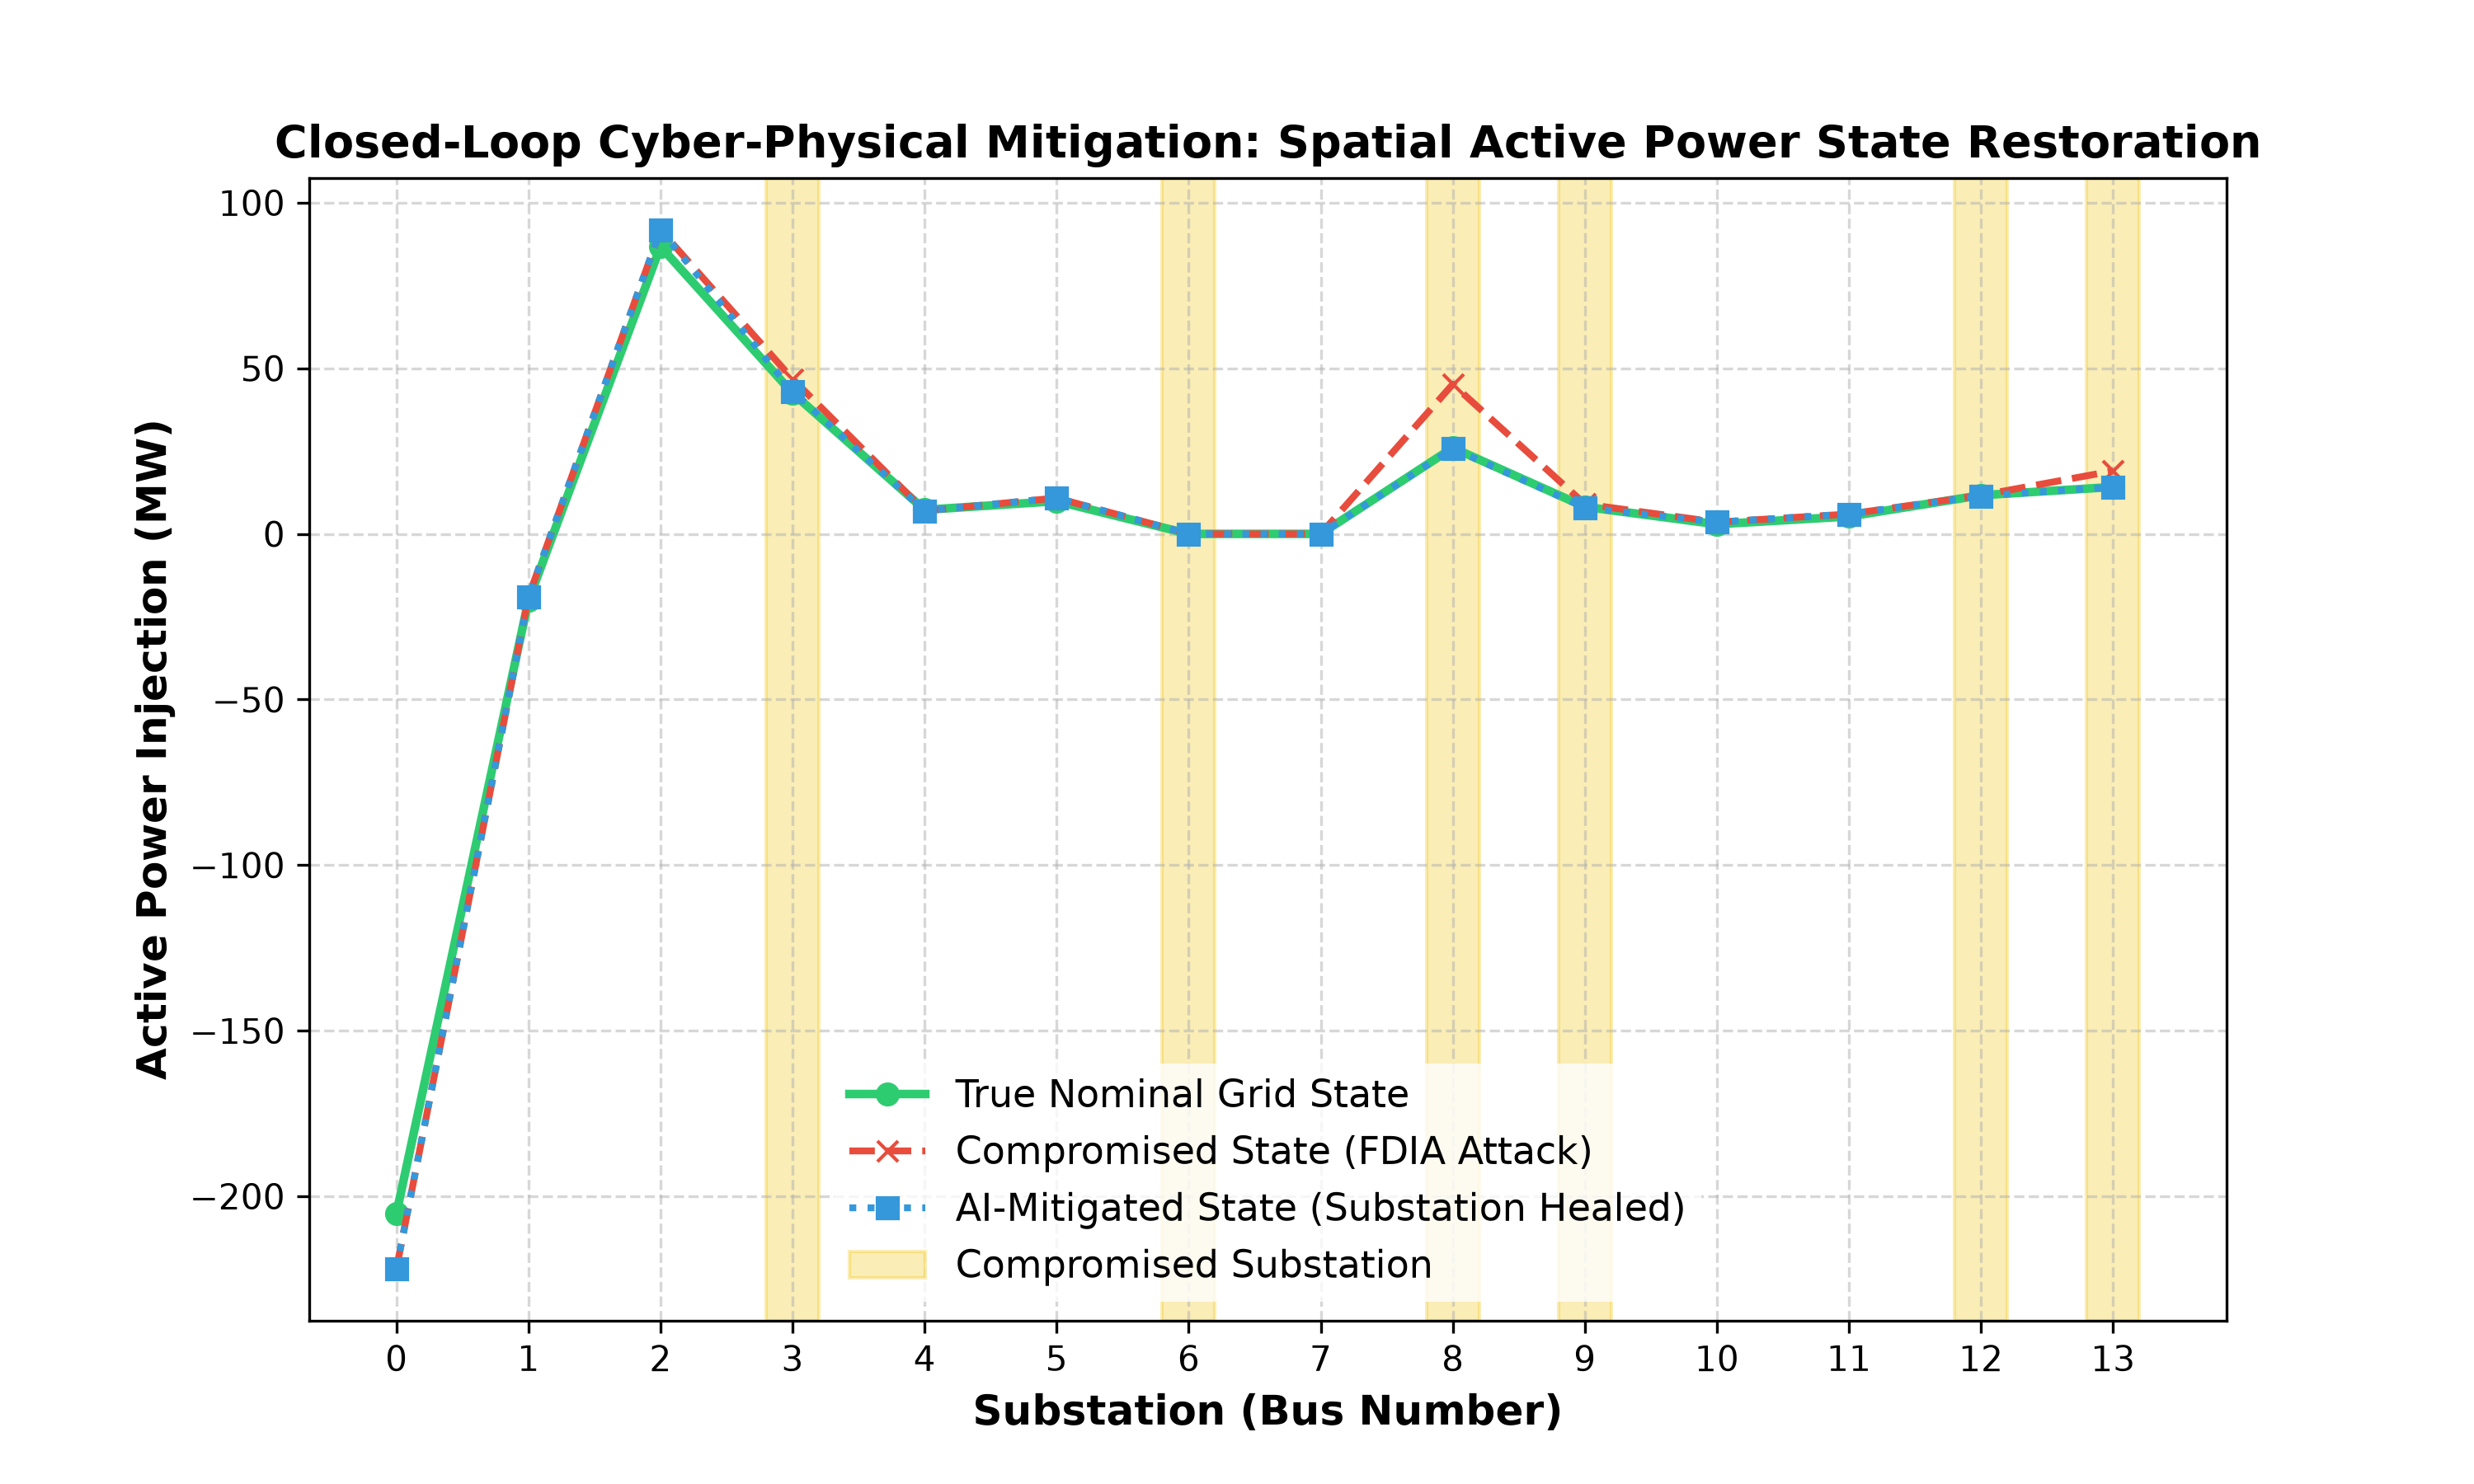
\includegraphics[width=0.85\textwidth]{cyber_mitigation_results}
\caption{Closed-loop physical grid healing active power tracking profile before, during, and after mitigation.}
\label{fig:cyber_healing}
\end{figure}

\section{Explainability Case Study}
To evaluate the feature attributions computed by Integrated Gradients (IG), we simulated a targeted attack on Bus 5. The IG engine calculates the attribution weights for all telemetry features ($V_i, \theta_i, P_i, Q_i$) across the grid. The highest attribution magnitude ($0.486$) was correctly mapped to the voltage angle feature ($\theta$) at Bus 5, identifying it as the main attack vector. The spatial distribution of attributions is visualized as an explainability heatmap in Figure \ref{fig:ig_explanation}.

\begin{figure}[htbp]
\centering
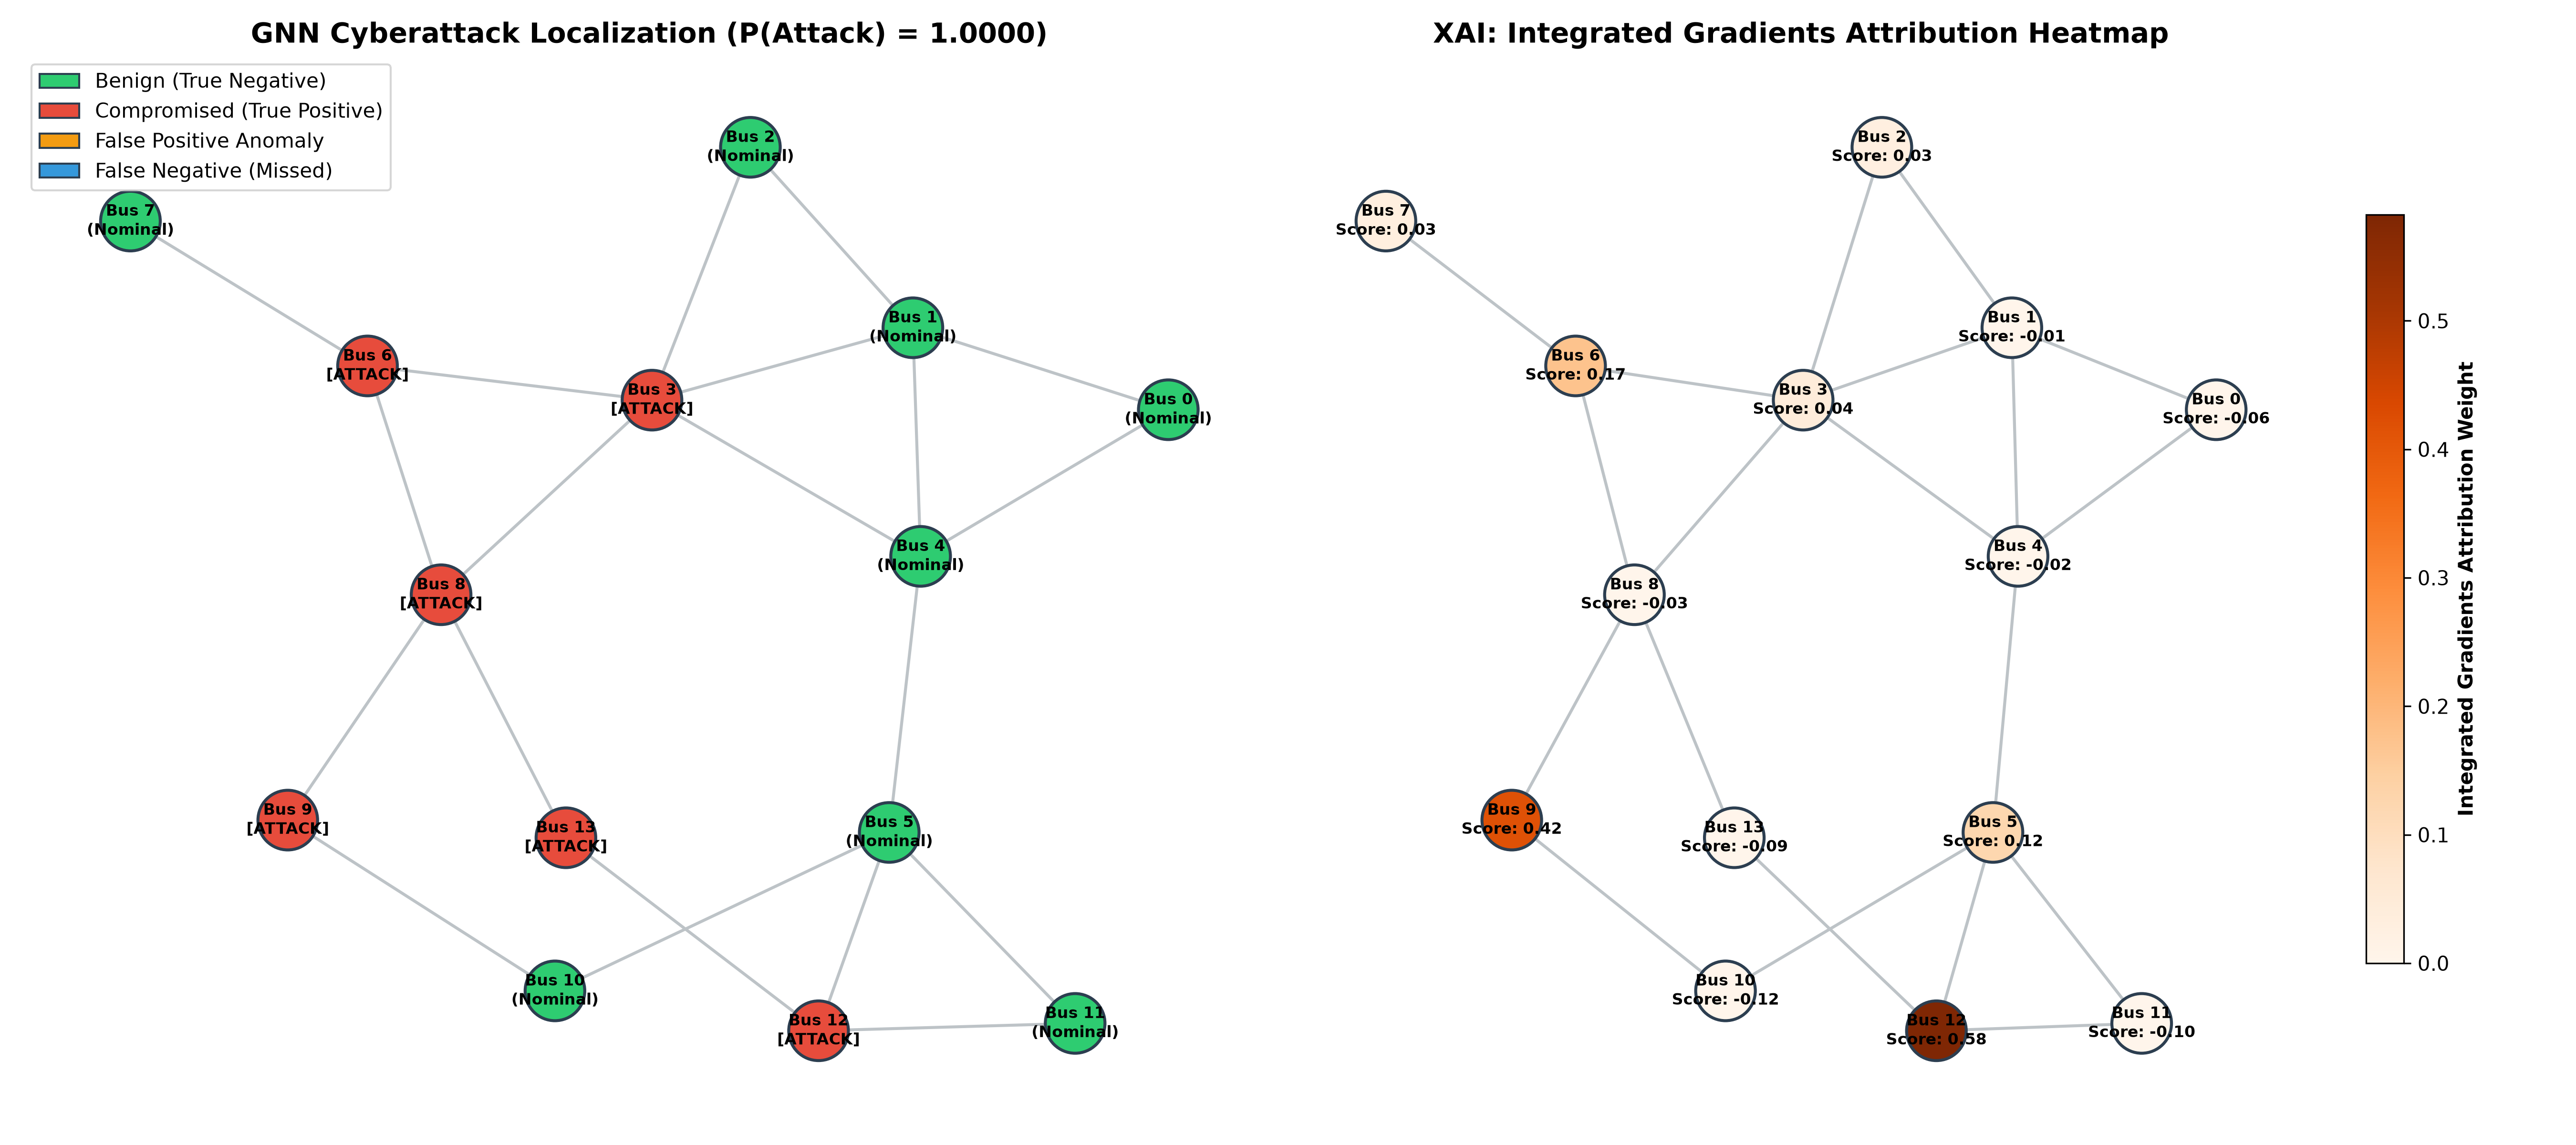
\includegraphics[width=0.85\textwidth]{grid_anomaly_explanation}
\caption{Integrated Gradients explainability heatmap illustrating telemetry feature attributions across buses.}
\label{fig:ig_explanation}
\end{figure}

%----------------------------------------------------------------------------------------
% CHAPTER 7: CONCLUSION
%----------------------------------------------------------------------------------------
\chapter{Conclusion \& Future Outlook}
This project report presented an explainable, topology-invariant Graph Digital Twin (GDT) framework for smart grid cybersecurity. By mapping SCADA telemetry onto a spatial graph and leveraging a joint multi-task GraphSAGE model, we achieved high-accuracy cyber-attack detection and localization. 

The concatenation-based spatial convolution successfully preserves local node feature signatures, mitigating over-smoothing. Integrated Gradients provides mathematically sound, sensor-level feature attributions to trace attack vectors. Under dynamic outages and scalability tests on the IEEE 30-bus grid, the GDT demonstrates superior generalization over flat classifiers. Finally, WLS benchmarks prove a $99.97\%$ tracking error reduction under active self-healing control.

Future work will expand the GDT framework by combining GraphSAGE with LSTMs to detect dynamic, slow-ramping anomalies, and validating the edge neighbor sampling scheme on large-scale transmission networks (e.g., IEEE 118-bus grid).

%----------------------------------------------------------------------------------------
% BIBLIOGRAPHY
%----------------------------------------------------------------------------------------
\begin{thebibliography}{00}
\bibitem{b1} N. E. M. Barreto and A. R. Aoki, ``Cyber-Physical Power System Digital Twins---A Study on the State of the Art,'' \emph{Energies}, vol. 18, no. 22, p. 5960, Nov. 2025.
\bibitem{b2} J. Sweeten et al., ``Cyber-Physical Fusion for GNN-Based Attack Detection in Smart Power Grids,'' \emph{IEEE Open Access Journal of Power and Energy}, vol. 12, pp. 288--299, Jun. 2025.
\bibitem{b3} Y. Liu, P. Ning, and M. K. Reiter, ``False data injection attacks against state estimation in electric power grids,'' \emph{ACM Transactions on Information and System Security}, vol. 14, no. 1, pp. 1--33, 2011.
\bibitem{b4} O. Kosut et al., ``Malicious data attacks on smart grid state estimation,'' \emph{IEEE Transactions on Smart Grid}, vol. 2, no. 4, pp. 662--673, Dec. 2011.
\bibitem{b5} J. Zhao and L. Mili, ``Robust state estimation against false data injection attacks in power systems,'' \emph{IEEE Transactions on Smart Grid}, vol. 8, no. 5, pp. 2452--2461, Sep. 2017.
\bibitem{b6} R. Deng, G. Xiao, and R. Lu, ``Defending against false data injection attacks on state estimation in smart grids: A survey,'' \emph{IEEE Transactions on Industrial Informatics}, vol. 13, no. 1, pp. 198--207, Feb. 2017.
\bibitem{b7} M. Sundararajan, A. Taly, and Q. Yan, ``Axiomatic attribution for deep networks,'' in \emph{Proc. ICML}, 2017, pp. 3319--3328.
\bibitem{b8} W. Hamilton, Z. Ying, and J. Leskovec, ``Inductive representation learning on large graphs,'' in \emph{Proc. NeurIPS}, 2017, pp. 1024--1034.
\bibitem{b9} G. Liang et al., ``A review of false data injection attacks against modern power systems,'' \emph{IEEE Transactions on Smart Grid}, vol. 8, no. 4, pp. 1630--1638, Jul. 2017.
\bibitem{b10} O. Boyaci et al., ``Joint Detection and Localization of Stealth False Data Injection Attacks in Smart Grids Using Graph Neural Networks,'' \emph{IEEE Transactions on Smart Grid}, vol. 13, no. 1, pp. 807--819, Jan. 2022.
\bibitem{b11} M. A. Rahman and H. Mohsenian-Rad, ``False data injection attacks with incomplete information against smart grid state estimation,'' \emph{IEEE Transactions on Smart Grid}, vol. 3, no. 4, pp. 2175--2183, Dec. 2012.
\bibitem{b12} M. He and J. Zhang, ``A Dependency Graph Approach for Fault Detection and Localization Towards Secure Smart Grid,'' \emph{IEEE Transactions on Smart Grid}, vol. 2, no. 2, pp. 342--351, Jun. 2011.
\bibitem{b13} A. Teixeira et al., ``Cyber-physical security of a smart grid infrastructure,'' \emph{Proceedings of the IEEE}, vol. 103, no. 10, pp. 2292--2313, Oct. 2015.
\bibitem{b14} X. Yue and G. Qu, ``Graph neural networks approach for cyberattack detection in smart grids,'' in \emph{Proc. CARS}, 2024, pp. 1--6.
\bibitem{b15} R. Ying et al., ``Gnnexplainer: Generating explanations for graph neural networks,'' in \emph{Proc. NeurIPS}, 2019, pp. 9240--9251.
\end{thebibliography}

\end{document}
